\documentclass[12pt,a4paper]{article}
\usepackage[utf8]{inputenc}

\usepackage{amsmath}
\usepackage{amsfonts}
\usepackage{amssymb}
\usepackage{graphicx}
\usepackage{listings}
\usepackage[margin=1.0in]{geometry}
\usepackage{caption}
\usepackage{subcaption}
\usepackage{float}
\usepackage[utf8]{inputenc}
\usepackage{refstyle}
\usepackage{spverbatim}
\usepackage{listings}
\usepackage{csvsimple}
\usepackage{adjustbox}
\usepackage{cancel}
\usepackage{scalerel,stackengine}
\usepackage[ruled,vlined]{algorithm2e}
\stackMath
\newcommand\reallywidehat[1]{%
\savestack{\tmpbox}{\stretchto{%
  \scaleto{%
    \scalerel*[\widthof{\ensuremath{#1}}]{\kern-.6pt\bigwedge\kern-.6pt}%
    {\rule[-\textheight/2]{1ex}{\textheight}}%WIDTH-LIMITED BIG WEDGE
  }{\textheight}% 
}{0.5ex}}%
\stackon[1pt]{#1}{\tmpbox}%
}
\parskip 1ex

\lstset{numbers=left,
	title=\lstname,
	numberstyle=\tiny, 
	breaklines=true,
	tabsize=4,
	language=Python,
	morekeywords={with,super,as},,
	frame=single,
	basicstyle=\footnotesize\tt,
	commentstyle=\color{comment},
	keywordstyle=\color{keyword},
	stringstyle=\color{string},
	backgroundcolor=\color{background},
	showstringspaces=false,
	numbers=left,
	numbersep=5pt,
	literate=
		{æ}{{\ae}}1
		{å}{{\aa}}1
		{ø}{{\o}}1
		{Æ}{{\AE}}1
		{Å}{{\AA}}1
		{Ø}{{\O}}1
	}

\usepackage{bm}
\PassOptionsToPackage{hyphens}{url}\usepackage{hyperref}
\usepackage[usenames, dvipsnames]{color}

\begin{document}

\begin{center}
\LARGE{\textbf{Project 2: Classification and Regression, from linear and logistic regression to neural networks}}
\\
\large{\textbf{Course: FYS-STK4155}}
\\
\large{\textbf{Semester: Autumn 2020}}
\\
\large{\textbf{Name: Sander Losnedahl}}
\end{center}

\begin{center}
\Large{\textbf{Abstract}}
\end{center}

\noindent a

\newpage

\begin{center}
\Large{\textbf{Introduction}}
\end{center}

\noindent This project first aims to solve the one dimensional heat equation (function of time and one direction in space) using both a forward Euler scheme and a neural network algorithm. The two solutions are then compared to the analytical solution to the heat equation. Then, the same neural network algorithm is slightly adjusted in order for the algorithm to find the eigenvector corresponding to the smallest (could also be the highest) eigenvalue of a $6*6$ real, symmetric and randomly generated matrix.
\\
We start by taking a look at the heat equation and finding an analytical solution to this partial differential equation. Then, a forward Euler scheme is proposed and implemented together with the analytical solution and the results of the two implementations are compared. The comparison is then repeated for different step sizes of the forward Euler scheme.
\\
Then, a dense neural network code is implemented in order to solve the heat equation using the Adam optimizer with Tensorflow. The algorithm itself is first discussed and the cost function is defined. The neural network solution of the implementation is then compared with the analytical solution.
\\
The report then considers a $6*6$ real, symmetric and randomly generated matrix where the goal is to find the smallest eigenvalue. The neural network algorithm previously mentioned is reused with slight adjustments and the resulting eigenvalue is compared with an eigenvalue obtained from a generic eigenvalue solver (numpy was used in this case).
\\
The results from both the heat equation solutions and the eigenvalue solver is then discussed further and a conclusion is drawn. Further work that can be done is then discussed as well. 

\newpage

\begin{center}
\Large{\textbf{Preliminaries}}
\end{center}

\noindent \textbf{The Github page} can be found at \href{{https://github.com/sanderwl/FYS-STK4155/tree/master/Project3}}{\nolinkurl{https://github.com/sanderwl/FYS-STK4155/tree/master/Project3}}. The report itself along with all the code and figures cna be found on this page.
\\
\textbf{Tensorflow} is a central Python package that is needed for the much of the neural network code in this project. I suggest you install Tensorflow with \textbf{Anaconda} as this proved much easier than with some other local interpreter.

\newpage

\begin{center}
\Large{\textbf{Exercise 1a): a}}
\end{center}

\begin{center}
\large{\textbf{Defining the heat equation}}
\end{center}

\noindent In this exercise we want to mathematically describe how heat can transfer within a rod of length L over a given time interval t. The rod will initially be heated at time $t = 0$ with some distribution, but after this point in time, the rod will cool off and the heat will decay as a function of time. How the heat changes as function of time and space is given by the heat equation as seen below.

\begin{equation}\label{eq:heatEquation}
\frac{\partial u(x,t)}{\partial t} = \frac{K_0}{c\rho} \frac{\partial^2 u(x,t)}{\partial x^2} 
\end{equation}

\noindent where $u(x,t)$ is the temperature at a specific time t and a position x. The term $\frac{K_0}{c\rho}$ is the thermal diffusivity which consists of thermal conductivity $K_0$ divided by the specific heat capacity c times the density of the material $\rho$ (KILDE). This quantity is a measure of the rate of heat transfer from the heated part of the rod to the cold part of the rod. 
\\
Equation \ref{eq:heatEquation} is a partial differential equation (PDE) which means that we need an initial condition and two boundary conditions in order to solve the equation. The initial condition can be interpreted as how much the rod is heated at $t = 0$ while the boundary conditions can be interpreted as how the heat reacts to the ends of the rod at $x = 0$ and $x = L$. The boundary conditions in this case is given by equations \ref{eq:boundary0} and \ref{eq:boundaryL}.

\begin{equation}\label{eq:boundary0}
u(0,t) = 0
\end{equation}

\begin{equation}\label{eq:boundaryL}
u(L,t) = 0
\end{equation}

\noindent We can set the initial condition such that the rod is heated the most at the middle and least at the ends. Such a condition can be described by a sine function as given in equation \ref{eq:initial}.

\begin{equation}\label{eq:initial}
u(x,0) = sin(\pi x)
\end{equation}

\noindent One can observe from equation \ref{eq:initial} that a rod of length 1 is heated the most at $L/2 = 0.5$ and is not heated at all at the ends of the rod. 

\begin{center}
\large{\textbf{Analytical solution to the heat equation}}
\end{center}

\noindent We can now split equation \ref{eq:heatEquation} into its spatial and temporal components such that 

\begin{equation}\label{eq:split}
u(x,t) = X(x)T(t)
\end{equation}

\noindent Equation \ref{eq:split} can then be solved for x and t respectively. We start by taking the partial derivatives of equation \ref{eq:split} with respect to both t and x.

\begin{equation}\label{eq:split2}
\begin{aligned}
u_t = X(x)T'(t)
\\
u_{xx} = X''(x)T(t)
\end{aligned}
\end{equation}

\noindent Equation \ref{eq:heatEquation} then takes the form

\begin{equation}\label{eq:heatSplit}
\begin{aligned}
u_t = u_{xx}
\\
X(x)T'(t) = X''(x)T(t)
\\
\frac{X''(x)}{X(x)} = \frac{T'(t)}{T(t)} = \lambda
\end{aligned}
\end{equation}

\noindent where $\lambda$ is some constant. We can first solve equation \ref{eq:heatSplit} for its spatial part X such that

\begin{equation}\label{eq:solveX}
\begin{aligned}
\frac{X''(x)}{X(x)} = \lambda
\\
X''(x) - \lambda X(x) = 0
\end{aligned}
\end{equation}

\noindent Equation \ref{eq:solveX} is recognized as a Sturm-Liouville problem when $\lambda$ represents the eigenvalues of equation \ref{eq:solveX} (Hancock, 2006). This means that the solutions to equation \ref{eq:solveX} is given by equation \ref{eq:eigenSol}.

\begin{equation}\label{eq:eigenSol}
X_n(x)= b_n sin(n\pi x)
\end{equation}

\noindent where n is an eigenfunction given by $n = \sqrt{\lambda}/\pi$ where $\lambda$ are the eigenvalues of the Sturm-Liouville problem. Solutions then arise at $\lambda = \pi^2 n^2$ and from equation \ref{eq:heatSplit} the solution with respect to $T'(t)$ is found.

\begin{equation}\label{eq:eigenSolT}
\begin{aligned}
\frac{T'(t)}{T(t)} = \lambda
\\
T'(t) = \lambda T(t)
\end{aligned}
\end{equation}

\noindent which has the solution

\begin{equation}\label{eq:realSolT}
T'(t) = e^{\pi^2 n^2 t}
\end{equation}

\noindent We can then find the solution for $u(x,t)$ by combining equation \ref{eq:eigenSol} and equation \ref{eq:realSolT} such that

\begin{equation}\label{eq:heatsol}
u_n(x,t) = b_n sin(n\pi x)e^{\pi^2 n^2 t}
\end{equation}

\noindent The subscript n denotes the individual eigenfunctions that solve the heat equation, however, most of them do not satisfy the initial condition in equation \ref{eq:initial}. The sum of these functions may satisfy the initial condition and thus, equation \ref{eq:heatsol} becomes

\begin{equation}\label{eq:sumN}
u_n(x,t) = \sum_{n=1}^{\infty} b_n sin(n\pi x)e^{\pi^2 n^2 t}
\end{equation}

\noindent One can observe from equation \ref{eq:sumN} that the exponential term decreases as n increases. Therefore, a reasonable approximation may be to only utilize the first term of the sum such that equation \ref{eq:sumN} can be written as

\begin{equation}\label{eq:finalSol}
u_n(x,t) = sin(\pi x)e^{\pi^2 t}
\end{equation}

\noindent where the constant $b_n$ has been set to one. This is the final solution of the heat equation that will be implemented in the code.

\newpage

\begin{center}
\Large{\textbf{Exercise 1b: A numerical approach to solving the heat equation}}
\end{center}

\begin{center}
\large{\textbf{The forward Euler approach}}
\end{center}

\noindent The heat equation is a partial differential equation that can be solved numerically using the forward Euler algorithm (sometimes referred to as the explicit Euler method). This algorithm aims to incrementally approximate the gradient of spatial and temporal parts of the heat equation by utilizing the definition of the derivative as seen in equations \ref{eq:gradT} and \ref{eq:gradx}.

\begin{equation}\label{eq:gradT}
u_t \approx \frac{u(x, t+\Delta t) - u(x,t)}{\Delta t}
\end{equation}

\begin{equation}\label{eq:gradx}
u_{xx} \approx \frac{u(x + \Delta x, t) - 2u(x,t) + u(x-\Delta x,t)}{\Delta x^2}
\end{equation}

\noindent where $\Delta x$ and $\Delta t$ represents the incremental step size in space or time respectively. Since the initial and boundary conditions are known, the forward Euler algorithm can incrementally approximate the change in heat from the middle of the rod and out towards the boundary. Equations \ref{eq:gradT} and \ref{eq:gradx} can be combined using the heat equation from equation \ref{eq:heatEquation} such that

\begin{equation}\label{eq:forwardEuler1}
\begin{aligned}
u_t = u_{xx}
\\
\frac{u(x,t+\Delta t) - u(x,t)}{\Delta t} = \frac{u(x+\Delta x, t)-2u(x,t)+u(x-\Delta x,t)}{\Delta x^2}
\\
\frac{u_j^{n+1}-u_j^n}{\Delta t} = \frac{u_{j+1}^n - 2u_j^n + u_{j-1}^2}{\Delta x^2}
\end{aligned}
\end{equation}

\noindent where the subscript j denotes the step in space and the subscript n denotes the step in time. We can solve equation \ref{eq:forwardEuler1} for $u_j^{n+1}$ such that we can calculate the heat incrementally forward in time. Thus, equation \ref{eq:forwardEuler1} becomes

\begin{equation}\label{eq:forwardEuler2}
\begin{aligned}
u_j^{n+1} = \Delta t(\frac{u_{j+1}^n - 2u_j^n + u_{j-1}^2}{\Delta x^2})+u_j^n
\\
u_j^{n+1} = (1-2\frac{\Delta t}{\Delta x^2})u_j^n + \frac{\Delta t}{\Delta x^2}(u_{j+1}^n + u_{j-1}^n)
\end{aligned}
\end{equation}

\noindent Equation \ref{eq:forwardEuler2} is only stable for $\frac{\Delta t}{\Delta x^2} \leq 0.5$, so the implementation needs to adjust $\Delta t$ according to $\Delta x$. The implementation of equation \ref{eq:forwardEuler2} allows us to solve the heat equation incrementally and the results are then compared to the analytical solution in the following section.

\begin{center}
\large{\textbf{Comparing the analytical and numerical solutions of the heat equation}}
\end{center}

\noindent We now compare how the heat translates throughout the rod at a given time for both the analytical implementation and for the forward Euler implementation. It was found that the heat decayed quickly as a result of the constant $b_n$ being set to zero in equation \ref{eq:finalSol}. Therefore, good time intervals of observing the heat was found to be at $t = 0$ (initial heat), $t = 0.5$ and $t = 1$. Figures \ref{fig:rodHeatEulerT0DX01}, \ref{fig:rodHeatEulerT05DX01} and \ref{fig:rodHeatEulerT1DX01} shows the heat distribution in the rod at these given times for $\Delta t = 0.005$ and $\Delta x = 0.1$ for both the analytical and forward Euler implementations (and their difference).

\begin{figure}[H]
\centering
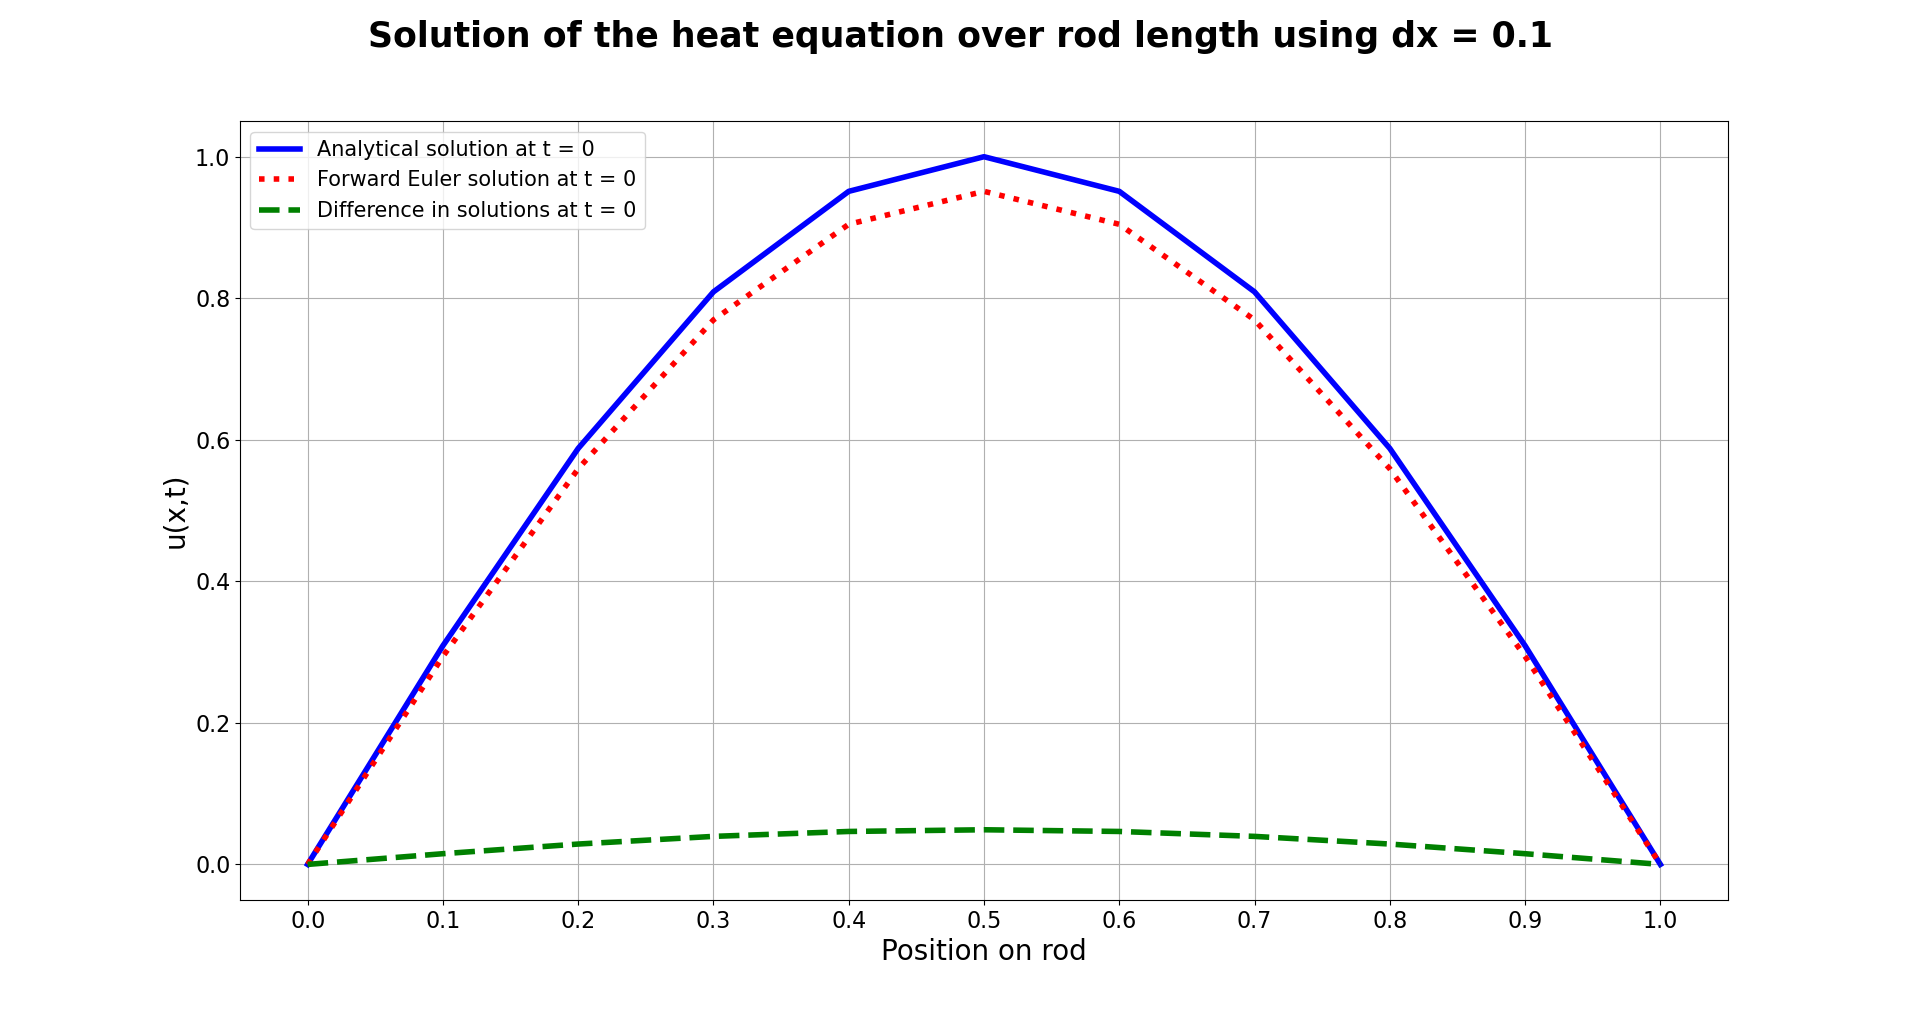
\includegraphics[width = 1\linewidth]{C:/Users/Sander/Documents/GitHub/FYS-STK4155/Project3/Report/Figures/Heat_Euler_t0_dx01.PNG}
\caption{\label{fig:rodHeatEulerT0DX01} Heat distribution within the rod for both analytical (blue) and forward Euler (red) implementations. The heat is measured at $t = 0$ using step sizes of $\Delta t = 0.005$ and $\Delta x = 0.1$.}
\end{figure}

\begin{figure}[H]
\centering
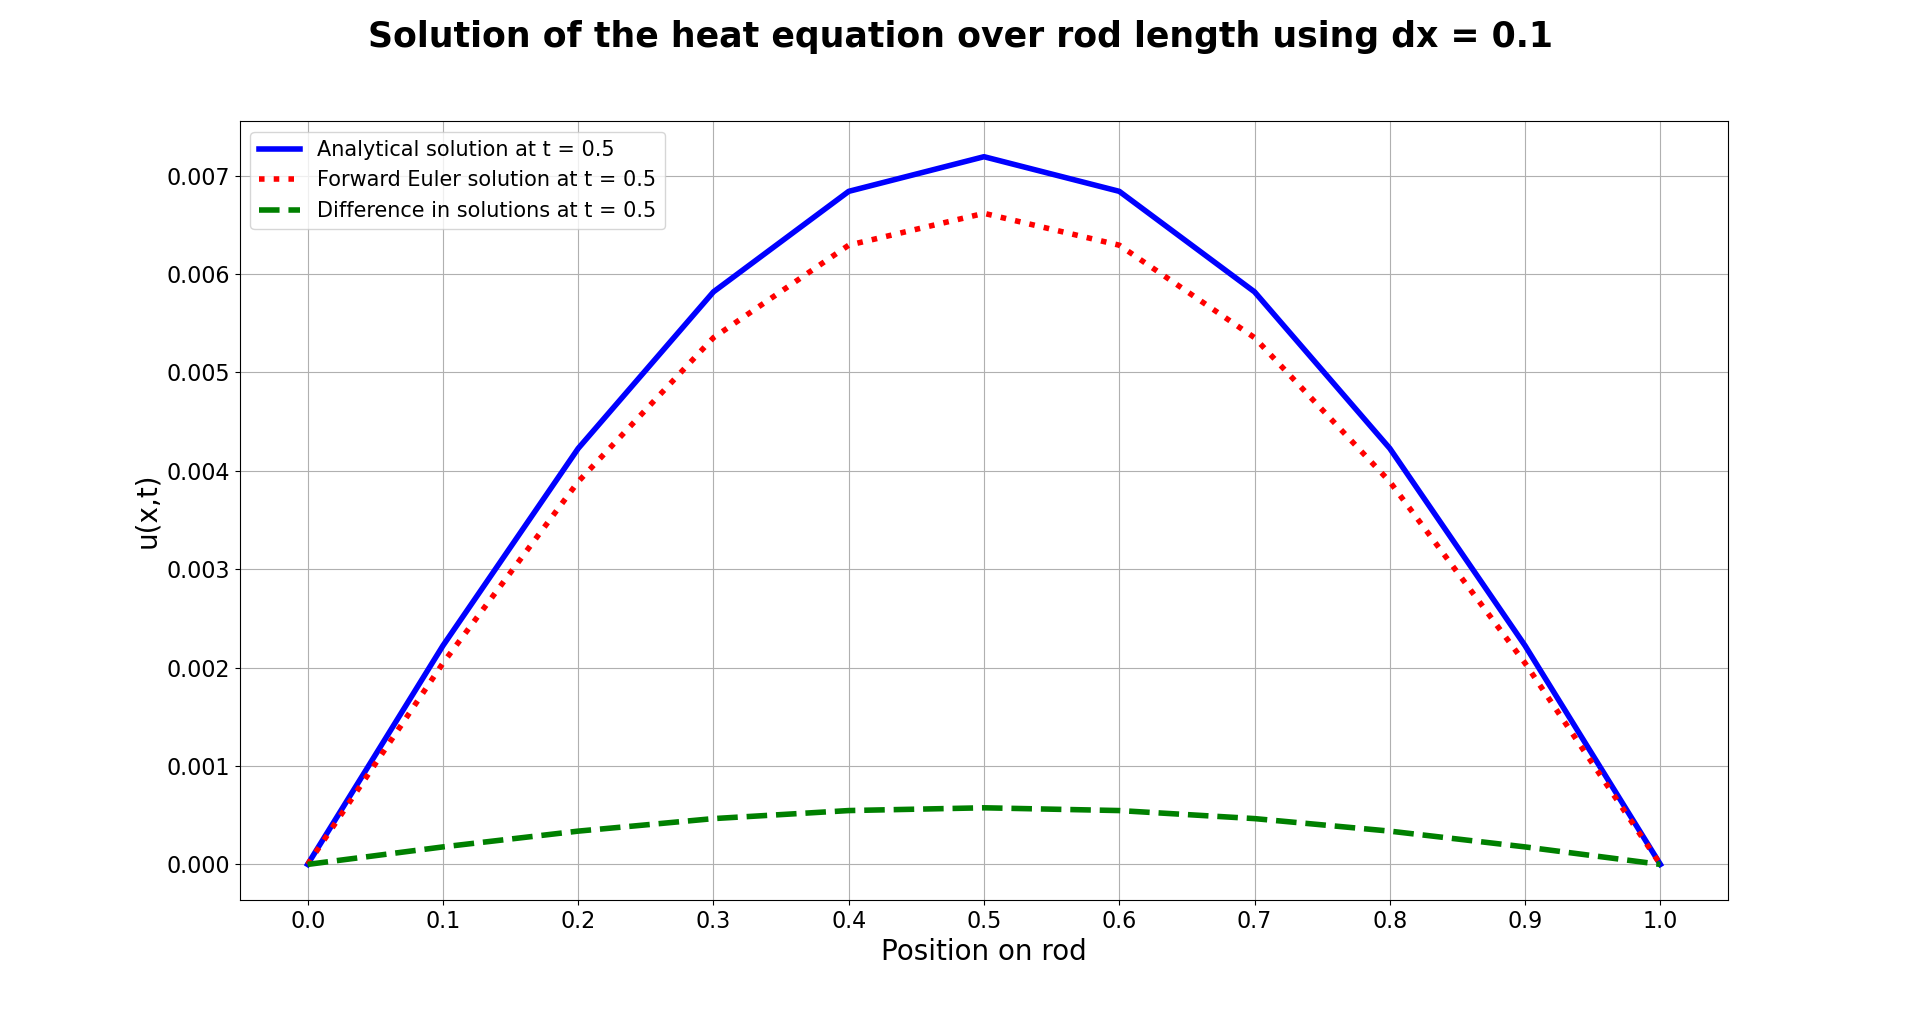
\includegraphics[width = 1\linewidth]{C:/Users/Sander/Documents/GitHub/FYS-STK4155/Project3/Report/Figures/Heat_Euler_t05_dx01.PNG}
\caption{\label{fig:rodHeatEulerT05DX01} Heat distribution within the rod for both analytical (blue) and forward Euler (red) implementations. The heat is measured at $t = 0.5$ using step sizes of $\Delta t = 0.005$ and $\Delta x = 0.1$.}
\end{figure}

\begin{figure}[H]
\centering
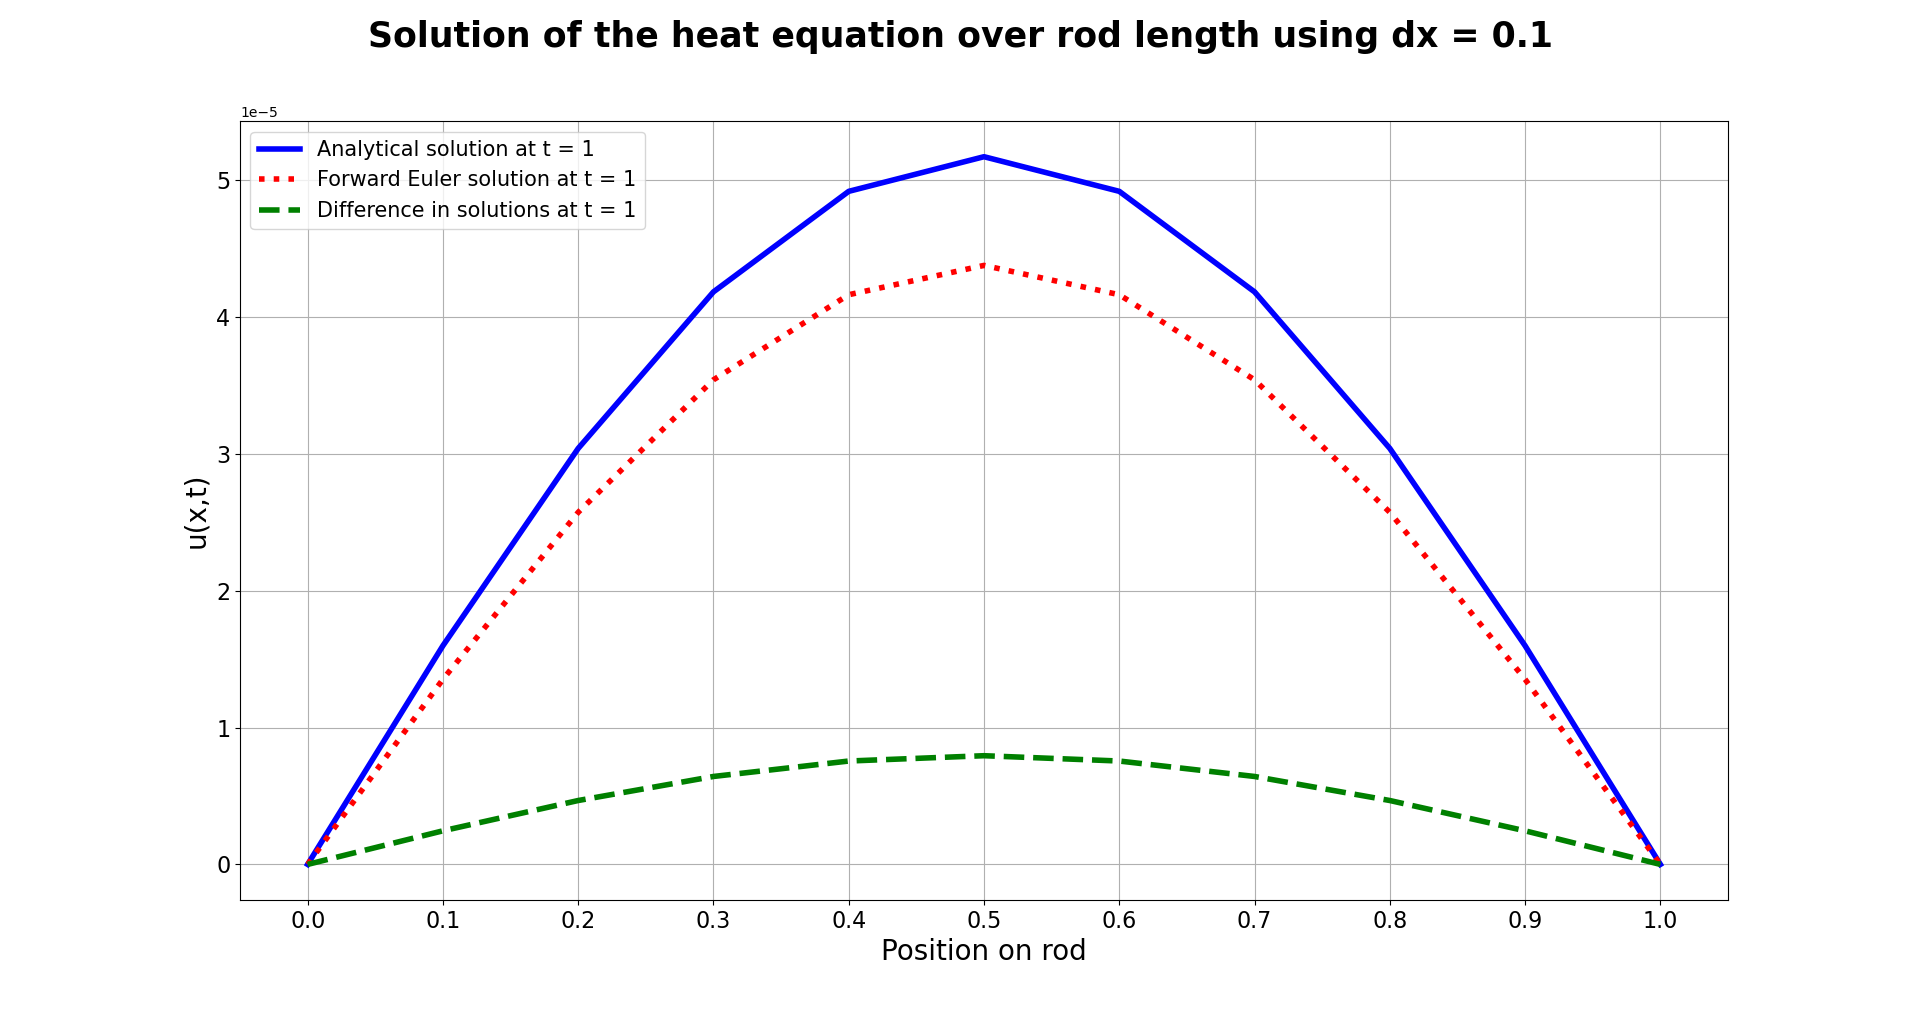
\includegraphics[width = 1\linewidth]{C:/Users/Sander/Documents/GitHub/FYS-STK4155/Project3/Report/Figures/Heat_Euler_t1_dx01.PNG}
\caption{\label{fig:rodHeatEulerT1DX01} Heat distribution within the rod for both analytical (blue) and forward Euler (red) implementations. The heat is measured at $t = 1$ using step sizes of $\Delta t = 0.005$ and $\Delta x = 0.1$.}
\end{figure}

\noindent One first observed that the rod is heated the most at the middle $x = 0.5$, which is according to the initial condition of equation \ref{eq:initial}. One can also observe that the forward Euler lies pretty close to the analytical solution. The difference between the analytical solution and the forward Euler solution decreases as time increases (the y-axis becomes smaller, so don't get fooled). Additionally, one can observe that the heat decays fairly quickly as most of the heat is gone within 1 second. 
\\
We now decrease the step size in space from $\Delta x = 0.1$ to $\Delta x = 0.01$, and this means that we need to adjust the step size in time according to $\frac{\Delta t}{\Delta x^2} \leq 0.5$. Therefore, the new step size in time becomes $\Delta t = 0.5*0.01^2 = 0.00005$. Figures \ref{fig:rodHeatEulerT0DX001}, \ref{fig:rodHeatEulerT05DX001} and \ref{fig:rodHeatEulerT1DX001} shows the same as the above figures, but using the new step sizes.

\begin{figure}[H]
\centering
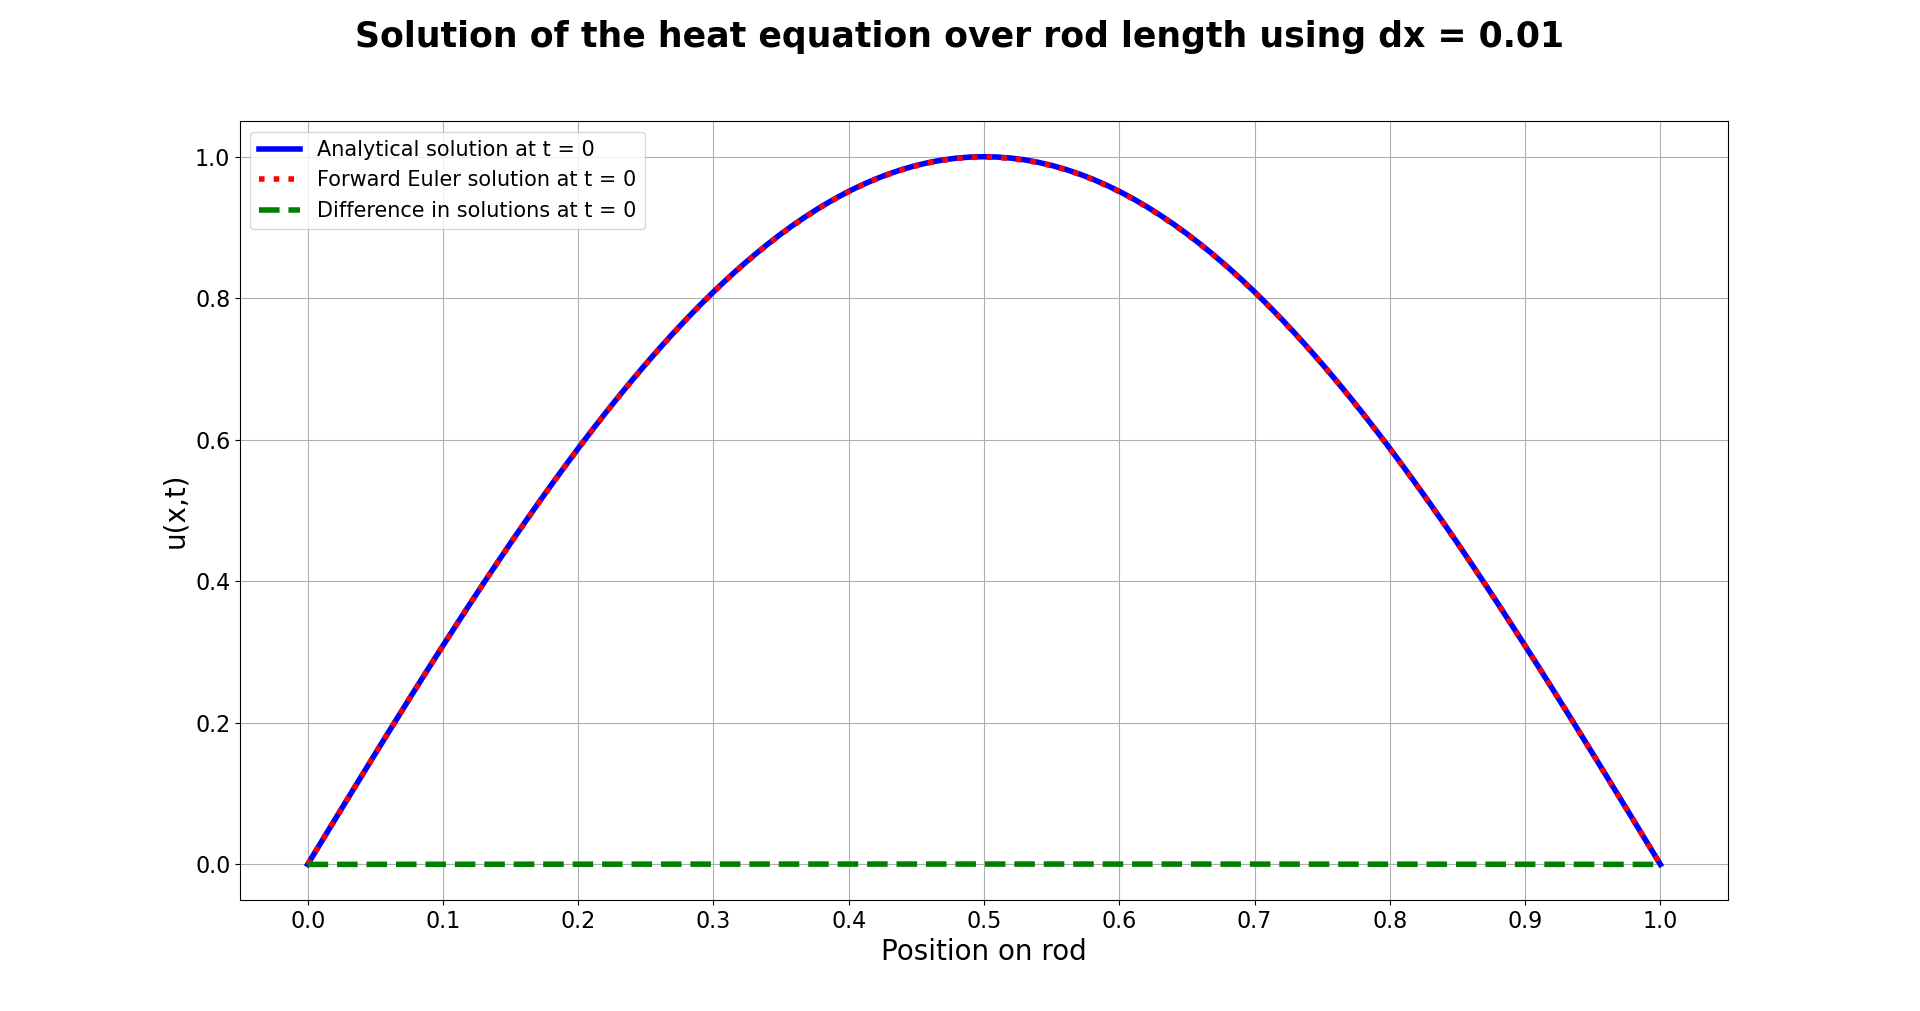
\includegraphics[width = 1\linewidth]{C:/Users/Sander/Documents/GitHub/FYS-STK4155/Project3/Report/Figures/Heat_Euler_t0_dx001.PNG}
\caption{\label{fig:rodHeatEulerT0DX001} Heat distribution within the rod for both analytical (blue) and forward Euler (red) implementations. The heat is measured at $t = 0$ using step sizes of $\Delta t = 0.00005$ and $\Delta x = 0.01$.}
\end{figure}

\begin{figure}[H]
\centering
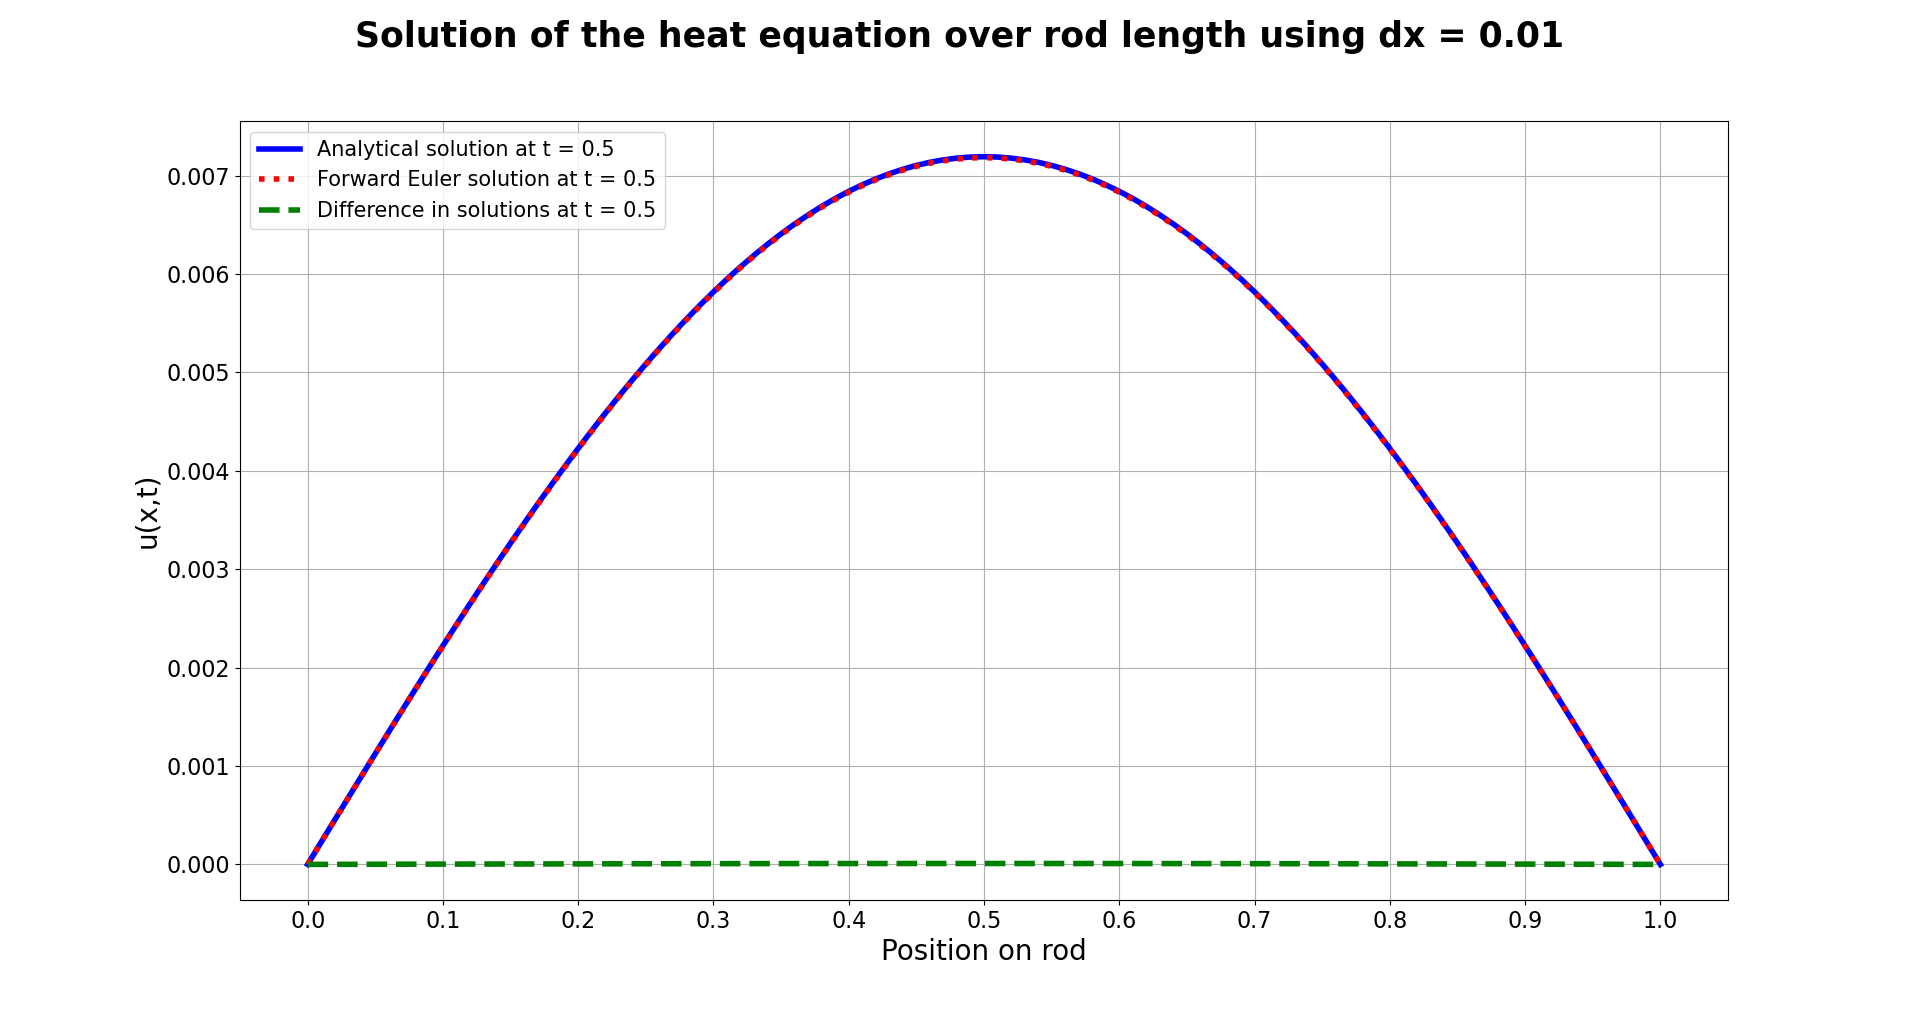
\includegraphics[width = 1\linewidth]{C:/Users/Sander/Documents/GitHub/FYS-STK4155/Project3/Report/Figures/Heat_Euler_t05_dx001.PNG}
\caption{\label{fig:rodHeatEulerT05DX001} Heat distribution within the rod for both analytical (blue) and forward Euler (red) implementations. The heat is measured at $t = 0.5$ using step sizes of $\Delta t = 0.00005$ and $\Delta x = 0.01$.}
\end{figure}

\begin{figure}[H]
\centering
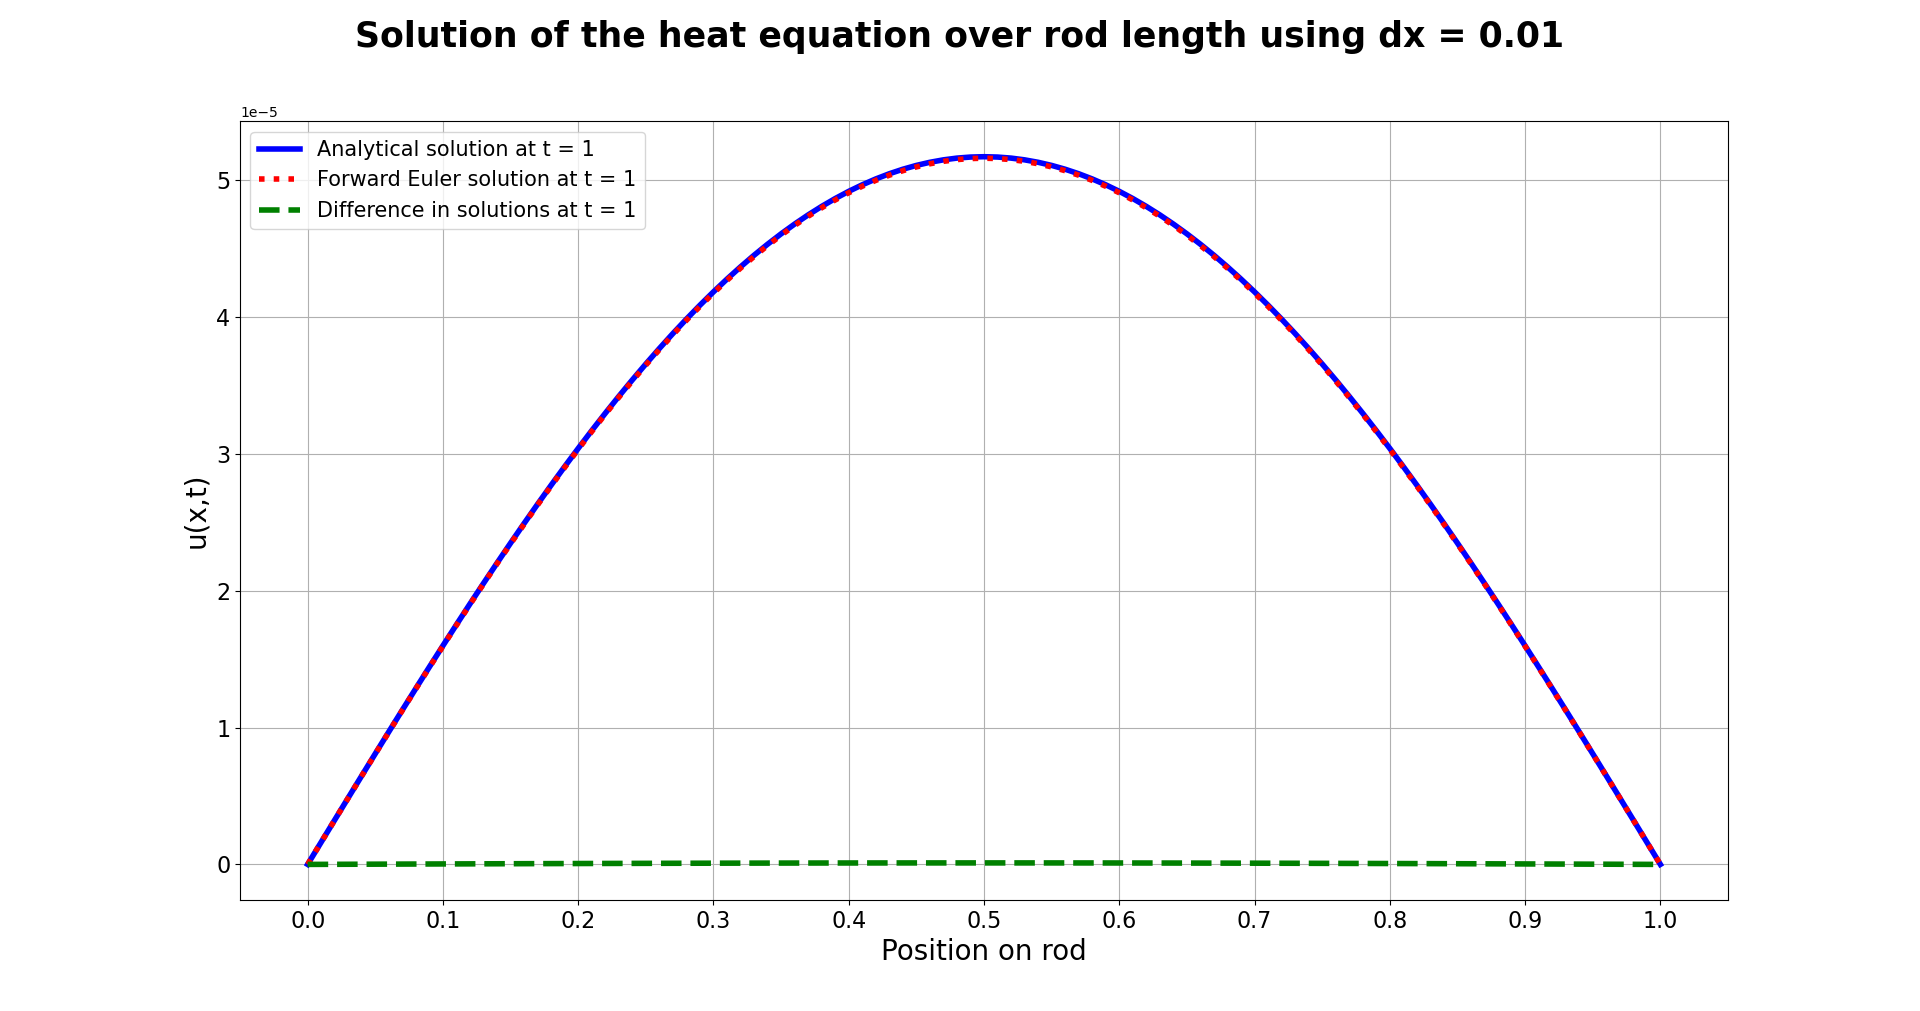
\includegraphics[width = 1\linewidth]{C:/Users/Sander/Documents/GitHub/FYS-STK4155/Project3/Report/Figures/Heat_Euler_t1_dx001.PNG}
\caption{\label{fig:rodHeatEulerT1DX001} Heat distribution within the rod for both analytical (blue) and forward Euler (red) implementations. The heat is measured at $t = 1$ using step sizes of $\Delta t = 0.00005$ and $\Delta x = 0.01$.}
\end{figure}

\noindent It is now observed that the forward Euler implementation matches the analytical implementation perfectly at all times. The reason for this is because the forward Euler is based on the definition of the derivative which becomes a better approximation of the true derivative when the step sizes are small. This means further that the forward Euler implementation can accurately represent the heat distribution within a rod at all times and places.

\newpage

\begin{center}
\Large{\textbf{Exercise c): Solving PDEs with deep neural networks}}
\end{center}

\begin{center}
\large{\textbf{Neural network implementation}}
\end{center}

\noindent The concepts and details of a neural network was discussed in Project 2 which can be found at \href{{https://github.com/sanderwl/FYS-STK4155/tree/master/Project2/Project2}}{\nolinkurl{https://github.com/sanderwl/FYS-STK4155/tree/master/Project2/Project2}}. Many of the concepts are the same, that is, we pass an input through a network of hidden layers and neurons and an output is produced. This process is then repeated where the goal is to minimize some cost function using gradient descent and weight updates. However, the implementation in this project is slightly different. 
\\
The neural network still aims to minimize some cost function which is this case is the MSE given by equation \ref{eq:MSE}.

\begin{equation}\label{eq:MSE}
\textrm{MSE} = \frac{1}{n} \sum_{i = 1}^n (\textrm{prediction error})^2
\end{equation}

\noindent Since $\frac{\partial u(x,t)}{\partial t} - \frac{\partial^2 u(x,t)}{\partial x^2} = 0$ solves the heat equation, it can be utilized as the prediction error. Equation \ref{eq:MSE} then becomes

\begin{equation}\label{eq:MSEHeat}
\textrm{MSE} = \frac{1}{n} \sum_{i = 1}^n (\frac{\partial u(x,t)}{\partial t} - \frac{\partial^2 u(x,t)}{\partial x^2})^2
\end{equation}

\noindent The goal of the neural network is to tune the weights such that the output matches the set of boundary conditions given in equations \ref{eq:boundary0} and \ref{eq:boundaryL}. For this, a trial solution is proposed. This solution is not guaranteed to minimize the cost function in equation \ref{eq:MSEHeat}, in fact, it is rare that such a solution minimize the cost function. Therefore, weights are tuned through gradient descent and different trial solutions are then proposed according to the current weights. For each update, the cost function gets closer to its minimal value and a more accurate solution to the heat equation is found. The trial solution g used in this project is given by equation \ref{eq:trial}.

\begin{equation}\label{eq:trial}
g = (1-t)*sin(\pi x) + x(1-x)t*\textrm{output}
\end{equation}

\noindent where $sin(\pi x)$ is the initial condition and output is the output from the neural network in which the gradient descent must handle. 
\\
The neural network is then trained by sending the two variables x and t through the network followed by a weight update through gradient descent on the cost function. This process happens many times and the final trial solution should reflect the analytical solution.

\begin{center}
\large{\textbf{Tensorflow implementation}}
\end{center}

\noindent A neural network algorithm was implemented from scratch using what I have learned in this course. However, this algorithm proved way too slow and was thus deemed unfit for this exercise as time is limited. Instead, Tensorflow algorithms were implemented as these yielded fast, stable and good results. Additionally, Tensorflow is easy to handle and has a lot of nice features to play around with. In particular, the Tensorflow version of the Adam optimization algorithm proved to yield great results. The Adam optimization algorithm is really a combinations of stochastic gradient descent with AdaGrad and RMSprop (Kingma and Ba, 2014). The algorithm is essentially stochastic gradient descent that utilizes both first and second moment adaptive learning rates (RMSProp) and scaling to the learning rate for each forward feed/back propagation (AdaGrad). The Adam has shown to be a robust and fast approach to deep learning, with some flaws, in the paper by Kingma and Ba (Kinga and Ba, 2014). The algorithm including the Adam optimization algorithm is described below.

\begin{algorithm}[H]
\SetAlgoLined
\KwResult{A trained model equivalent to solving the heat equation}
 Declare x and t in the Tensorflow format\;
 Define the cost function according to equations \ref{eq:MSEHeat} and \ref{eq:trial}\;
 Set up the dense layered neural network with the Adam optimizer\;
 \For{iterations}{
  Feed forward of x and t\;
  Gradient descent on the cost function with Adam optimizer\;
  Back propagation to update weights\;
  }
  Compare neural network result with the analytical
 \caption{Neural network algorithm}
\end{algorithm}

\noindent The above algorithm needs some input parameters which are defined in table \ref{tab:NNparams}.

\begin{table}[h]
\caption{\label{tab:NNparams} Parameters of the neural network.}
\centering
\begin{tabular}{|c|c|}
\hline
$\Delta$ t & $0.1$\\
\hline
$\Delta$ x & $0.1$\\
\hline
Number of layers & $3$\\
\hline
Number of neurons in each layer & $10$\\
\hline
Number of iterations & $1000000$\\
\hline
Initial learning rate & $0.001$\\
\hline
\end{tabular}
\end{table}

\noindent Since we are doing a stochastic gradient descent like algorithm (Adam optimizer) we have to set some initial learning rate. The number of iterations denotes how many times we do the feed forward/back propagation loop. The other parameters were found through trial and error. These parameters could have been optimized like in Project 2, but the results have shown to be good without exact optimization.

\begin{center}
\large{\textbf{Comparing the analytical and neural network solutions of the heat equation}}
\end{center}

\noindent After training the neural network as described in algorithm 1 with the parameters from table \ref{tab:NNparams}, we can pass x and t through the trained model and the final trial solution such that the output is equivalent with solving the heat equation. When this is done, the two-dimensional heat distribution (time and one spatial dimension) can be plotted as done in figures \ref{fig:3dHeatAna} and \ref{fig:3dHeatNN}.

\begin{figure}[H]
\centering
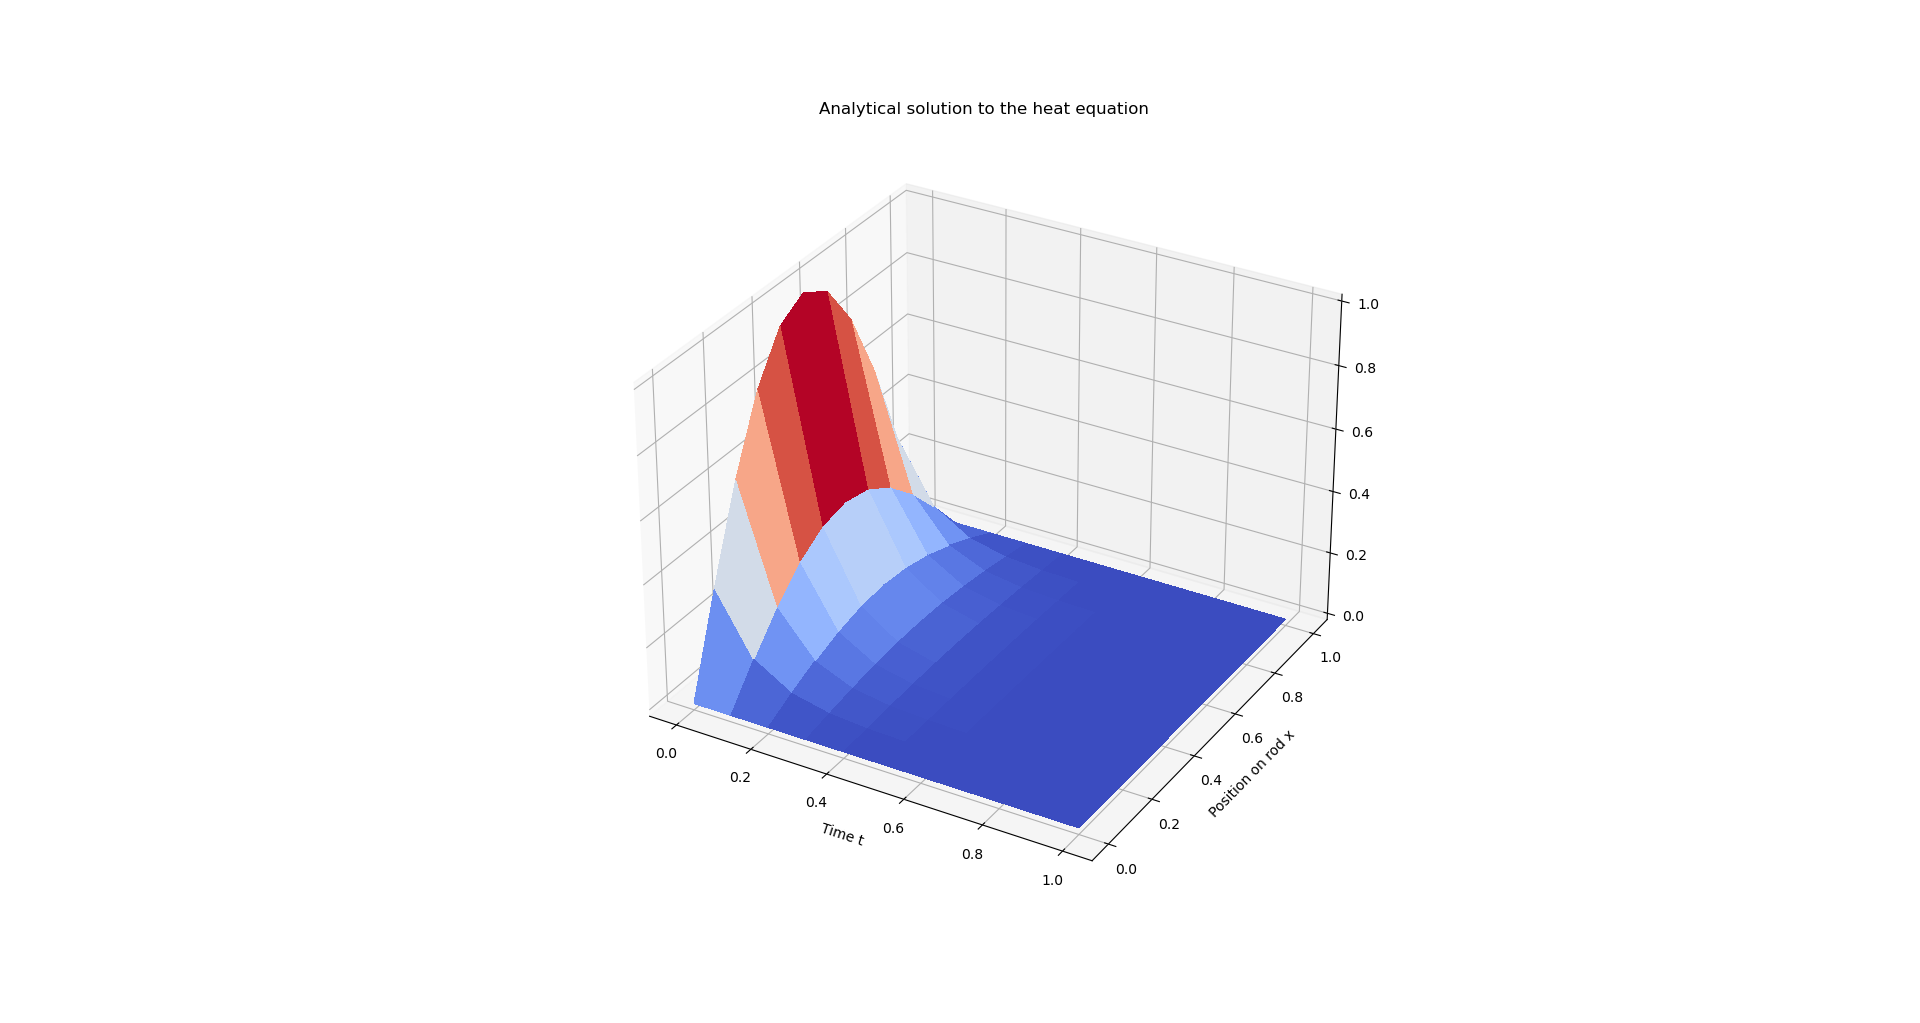
\includegraphics[width = 1\linewidth]{C:/Users/Sander/Documents/GitHub/FYS-STK4155/Project3/Report/Figures/3dHeat_ana.PNG}
\caption{\label{fig:3dHeatAna} Heat distribution for the rod as function of space and time for the analytical implementation.}
\end{figure}

\begin{figure}[H]
\centering
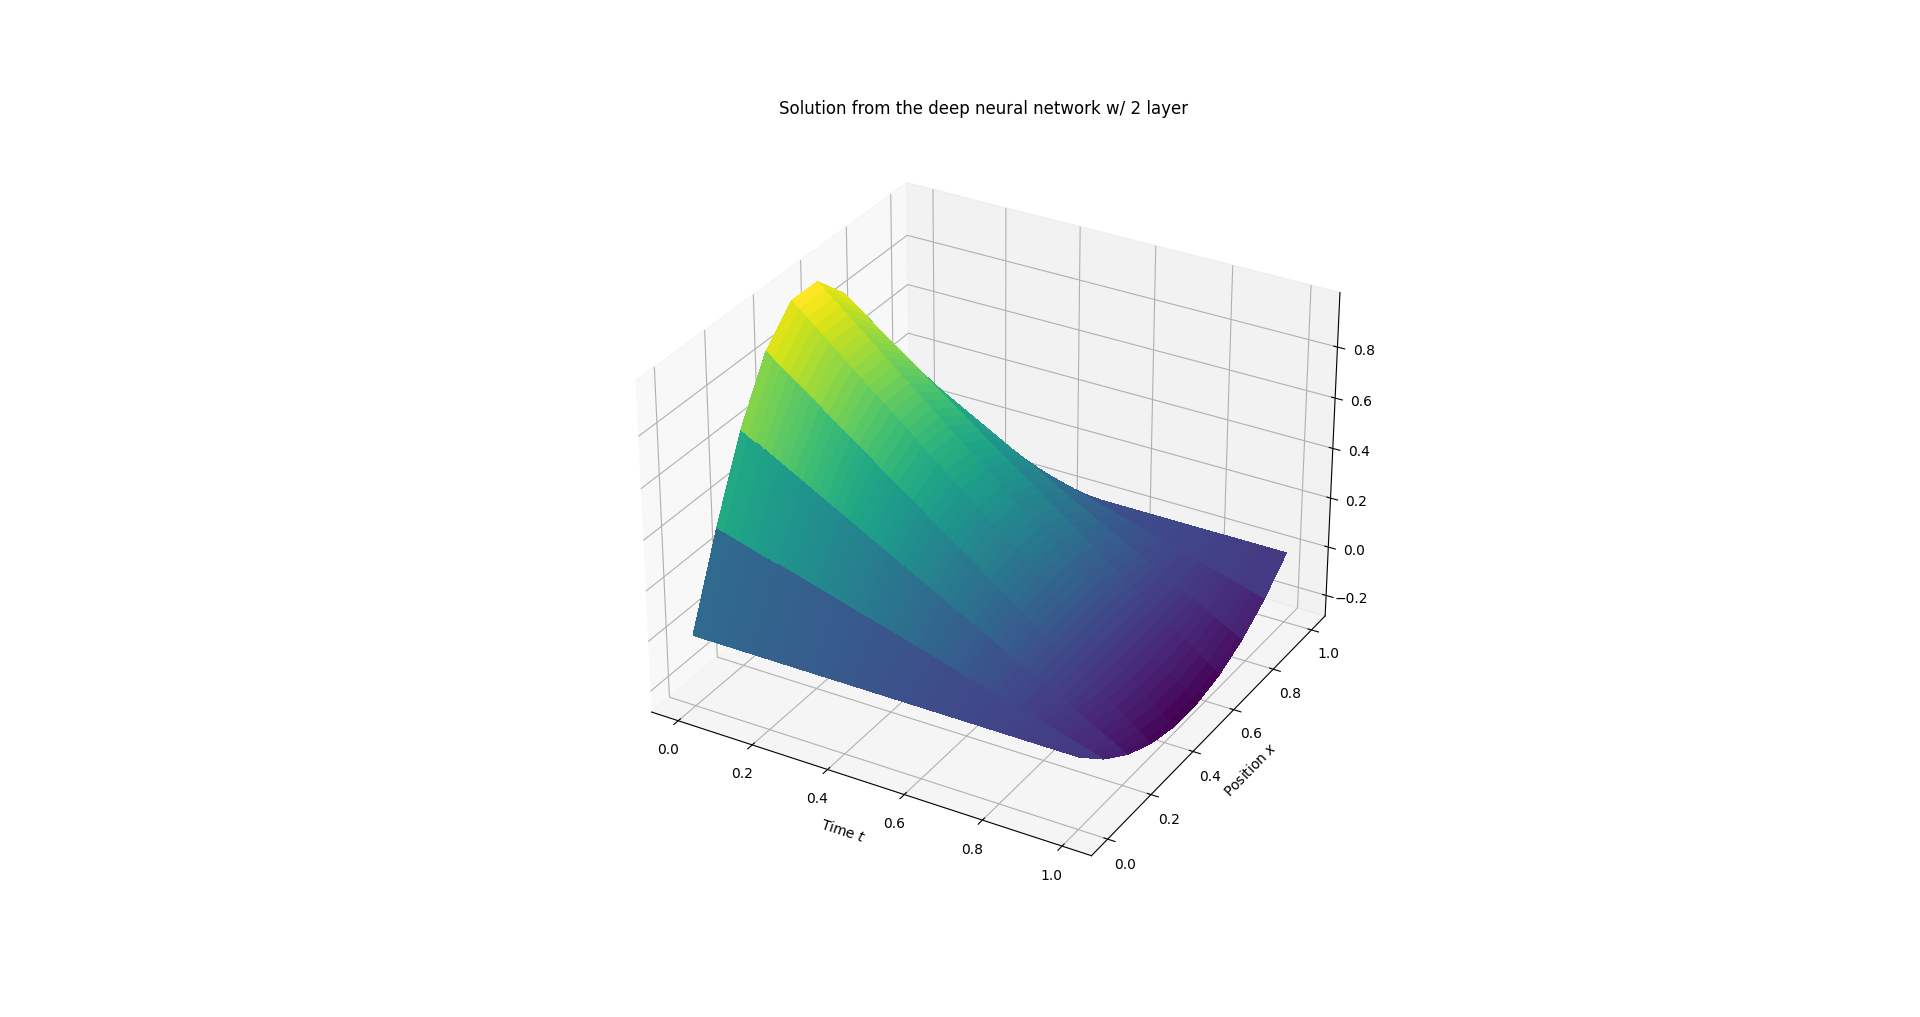
\includegraphics[width = 1\linewidth]{C:/Users/Sander/Documents/GitHub/FYS-STK4155/Project3/Report/Figures/3dHeat_NN.PNG}
\caption{\label{fig:3dHeatNN} Heat distribution for the rod as function of space and time for the neural network implementation.}
\end{figure}

\noindent One can observe that the two implementations in figures \ref{fig:3dHeatAna} and \ref{fig:3dHeatNN} are pretty similar. In order to get a better comparison, we can plot the heat distribution at constant times $t = 0$ (initial heat), $t = 0.5$ and $t = 1$ just like before.

\begin{figure}[H]
\centering
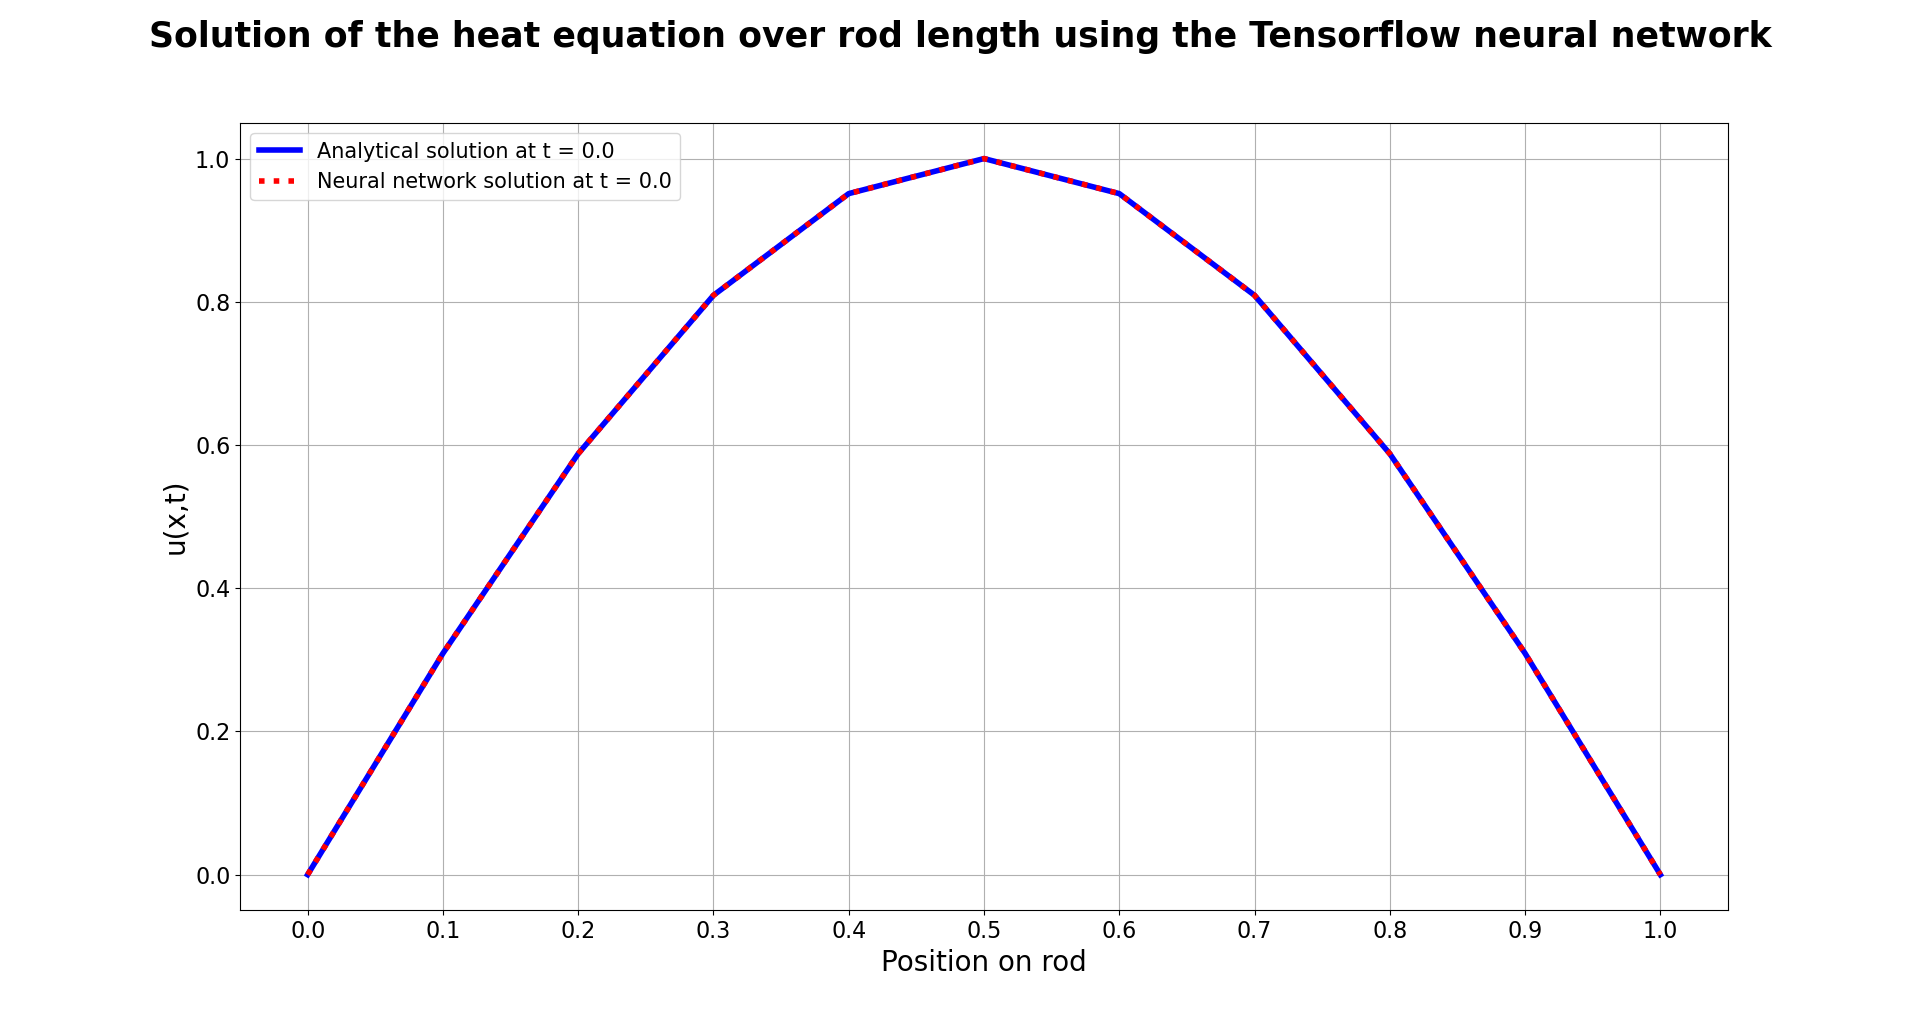
\includegraphics[width = 1\linewidth]{C:/Users/Sander/Documents/GitHub/FYS-STK4155/Project3/Report/Figures/Heat_TF_t0.PNG}
\caption{\label{fig:rodHeatTF0} Heat distribution within the rod for both analytical (blue) and neural network (red) implementations. The heat is measured at $t = 0$ using the parameters of table \ref{tab:NNparams}.}
\end{figure}

\begin{figure}[H]
\centering
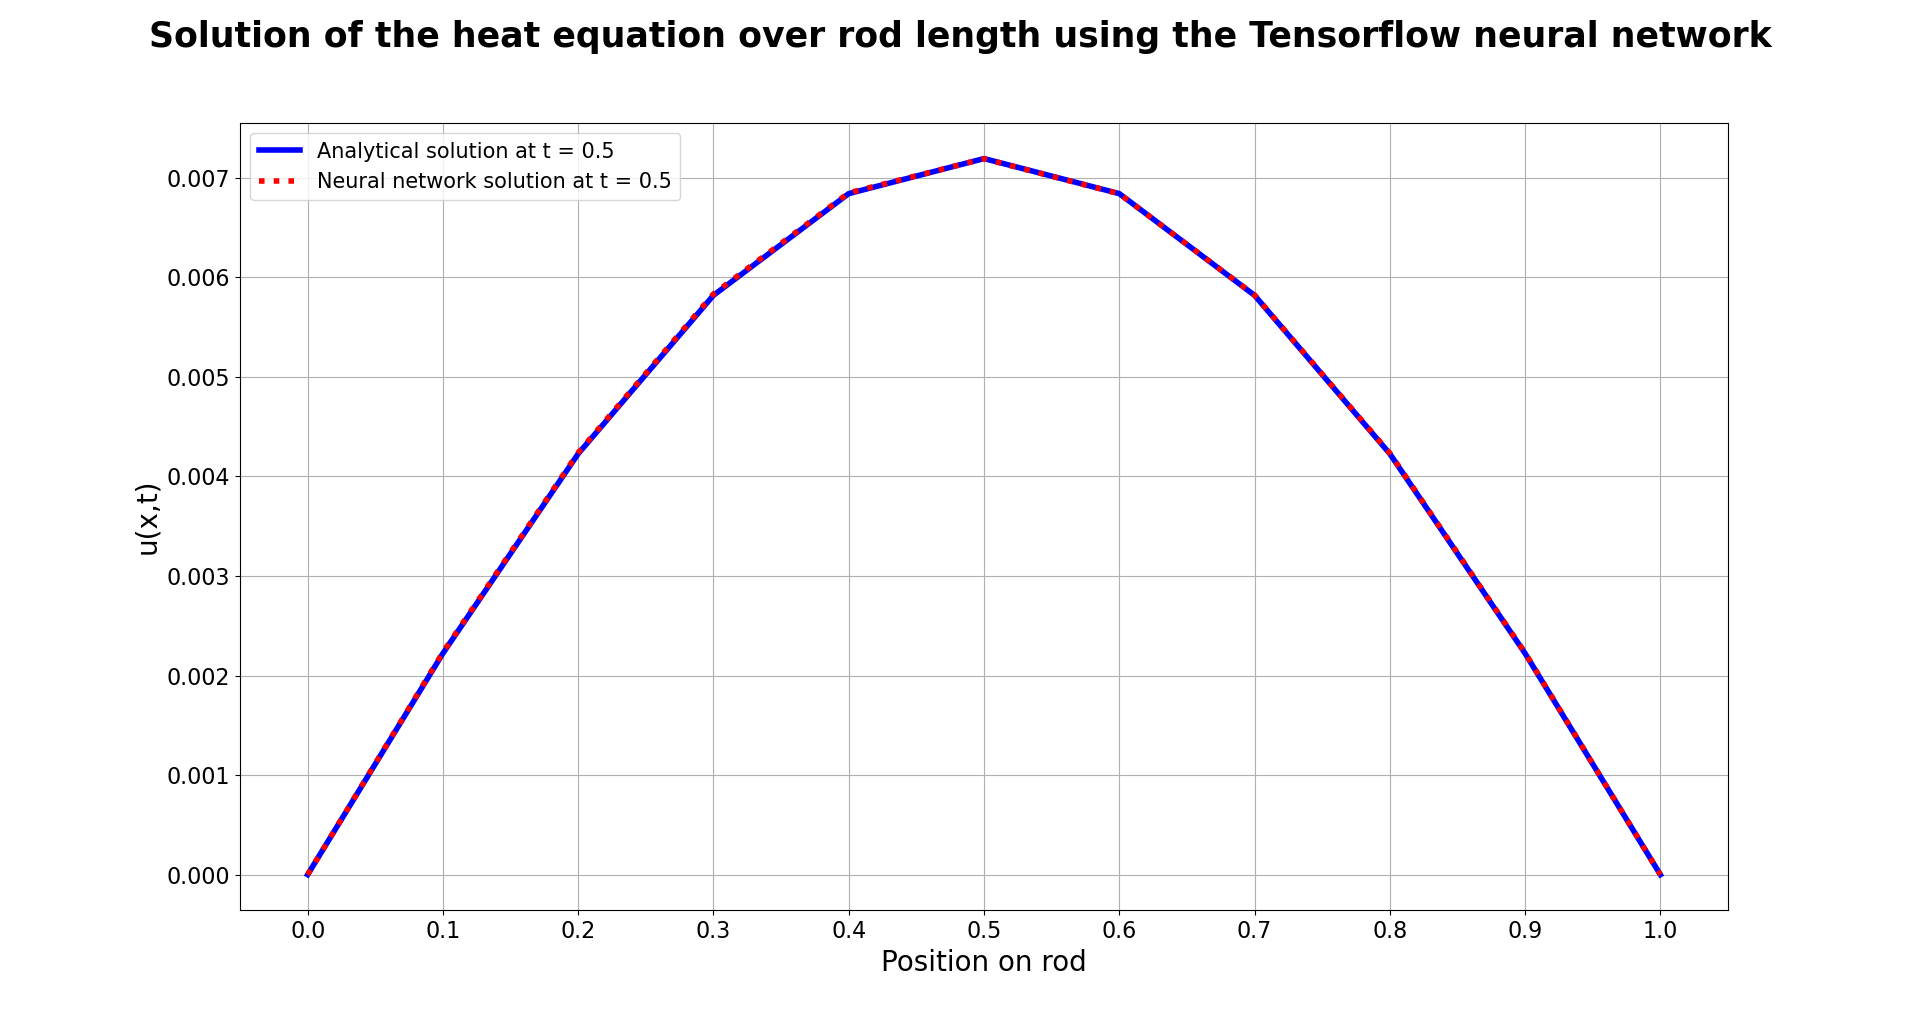
\includegraphics[width = 1\linewidth]{C:/Users/Sander/Documents/GitHub/FYS-STK4155/Project3/Report/Figures/Heat_TF_t05.PNG}
\caption{\label{fig:rodHeatTF05} Heat distribution within the rod for both analytical (blue) and neural network (red) implementations. The heat is measured at $t = 0.5$ using the parameters of table \ref{tab:NNparams}.}
\end{figure}

\begin{figure}[H]
\centering
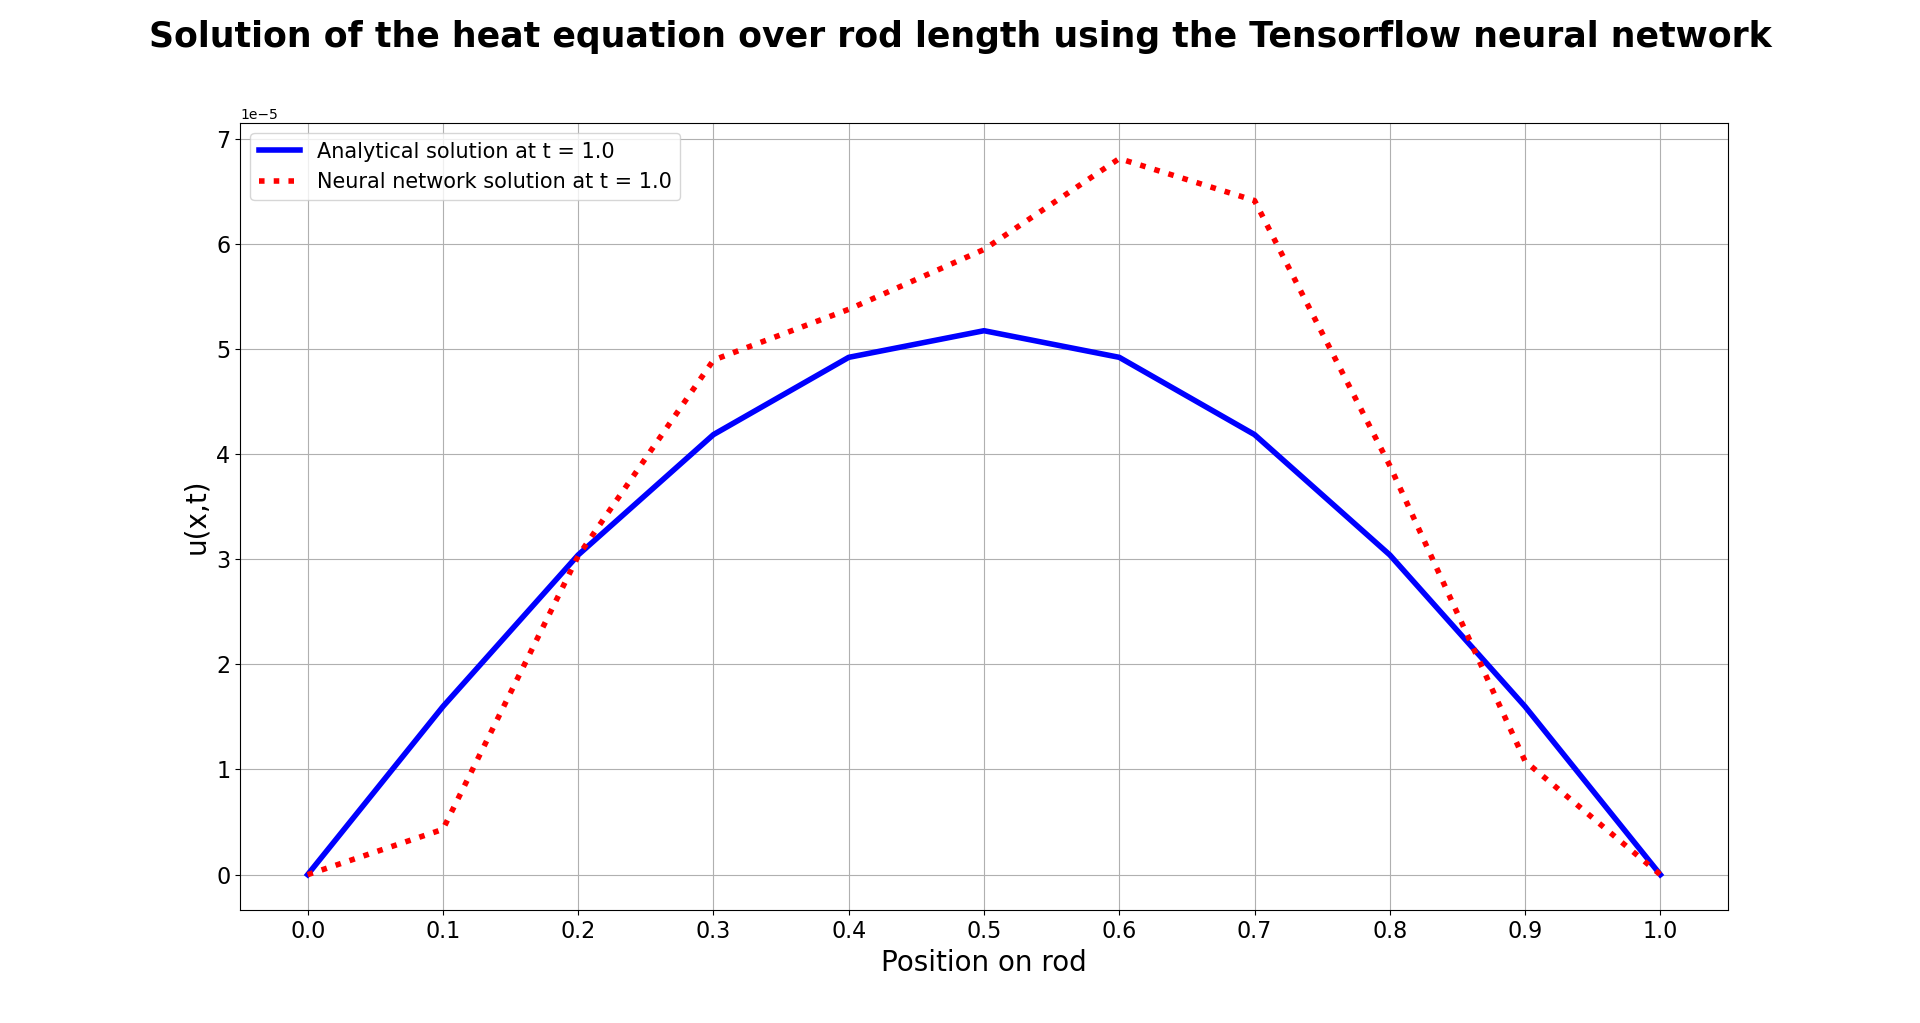
\includegraphics[width = 1\linewidth]{C:/Users/Sander/Documents/GitHub/FYS-STK4155/Project3/Report/Figures/Heat_TF_t1.PNG}
\caption{\label{fig:rodHeatTF1} Heat distribution within the rod for both analytical (blue) and neural network (red) implementations. The heat is measured at $t = 1$ using the parameters of table \ref{tab:NNparams}.}
\end{figure}

\noindent One can observe that the initial heat distribution in figure \ref{fig:rodHeatTF0} is equal for the analytical and neural network implementations. After $0.5$ seconds, the two implementations are still equivalent. At $t = 1$ however, the two implementations are essentially zero, but the neural network has now deviated from the analytical solution. This was a recurring problem with the neural network implementation regardless of input parameters. When the temperature started to approach zero, the neural network increasingly deviated from the analytical solution. However, since the deviation is very small, the result is deemed acceptable. Additionally, one can observe that the temperature at the different times are equivalent to the ones found by the forward Euler scheme.

\newpage

\begin{center}
\Large{\textbf{Exercise d): Eigenvectors and eigenvalues using neural networks}}
\end{center}

\begin{center}
\large{\textbf{Neural network implementation of eigenvector/value solver}}
\end{center}

\noindent In this exercise we aim to find the lowest (or highest) eigenvalue with a method proposed by Yi and Fu in the paper \emph{Neural Networks Based Approach Computing Eigenvectors and Eigenvalues of Symmetric Matrix} (Yi and Fu, 2004). The method utilizes a neural network set up similar to what is implemented in the previous exercise, but with a cost function given by equation \ref{eq:yiCost}.

\begin{equation}\label{eq:yiCost}
\frac{d x(t)}{dt} = -x(t) + f(x(t))
\end{equation}

\noindent where $x(t)$ is the state of the network (where and when the input is propagated through the network) and $f(x(t))$ is given by 

\begin{equation}\label{eq:fxt}
f(x(t)) = [x^TxA + (1-x^TAx)I]x
\end{equation}

\noindent Here, A is a real, symmetric and square matrix, I is the identity matrix and T marks the transpose. A is in this case defined by $k(Q^T + Q)/2$ which ensures symmetry, where Q is a real, randomly generated matrix. k is in this case either $-1$ or $1$ where $k = -1$ yields the smallest eigenvalue of the matrix and $k = 1$ yields the largest eigenvector of the matrix. 
\\
Most of the neural network code is reused from the previous exercise as described by algorithm 1, but the cost function is changes to equation \ref{eq:yiCost}. Additionally, we utilize the input parameters of table \ref{tab:NNparams}, but with $10$ layers instead of $3$ as this yielded better results. The algorithms stops iterating if the cost function is less that some threshold set to $0.00001$ in this case. The threshold is very low because the neural network results showed to be very sensitive to errors larger than this threshold.
\\
The matrix A was randomly generated and was in this run set to

\[
A=
  \begin{bmatrix}
    0.07630829 & 0.64051963 & 0.40967518 & 0.8273356 & 0.94355894 & 0.37167248 \\
    0.64051963 & 0.07205113 & 0.16718766 & 0.26239086 & 0.40619972 & 0.64725246 \\
    0.40967518 & 0.16718766 & 0.2881456 & 0.75507122 & 0.36839897 & 0.41225433 \\
    0.8273356 & 0.26239086 & 0.75507122 & 0.9501295 & 0.49035637 & 0.51294554 \\
    0.94355894 & 0.40619972 & 0.36839897 & 0.49035637 & 0.66901324 & 0.41682162 \\
    0.37167248 & 0.64725246 & 0.41225433 & 0.51294554 & 0.41682162 & 0.83791799 
  \end{bmatrix}
\]

\noindent which is a real and symmetric, square matrix. Running the neural network with $k = -1$ then yields an eigenvector $\nu_{min}$ corresponding to the lowest eigenvalue $\lambda_{min}$ of 

\begin{equation}\label{eq:minEigenVec}
\nu_{min}=[-0.51370594, -0.35445244, -0.39575076, -0.60860367, -0.51998609, -0.48656764]
\end{equation}

\noindent and a normalized eigenvector of

\begin{equation}\label{eq:minEigenVecNorm}
\nu_{min, norm}=[-0.43053478, -0.29706509, -0.33167704, -0.51006817, -0.43579814, -0.40779028]
\end{equation}

\noindent with a corresponding eigenvalue of 

\begin{equation}\label{eq:minEigenVal}
\lambda_{min} = 3.1220778592498455
\end{equation}

\noindent The neural network gets closer and closer to the correct eigenvector/eigenvalue for each iteration and figure \ref{fig:eigen1} shows exactly this convergence.

\begin{figure}[H]
\centering
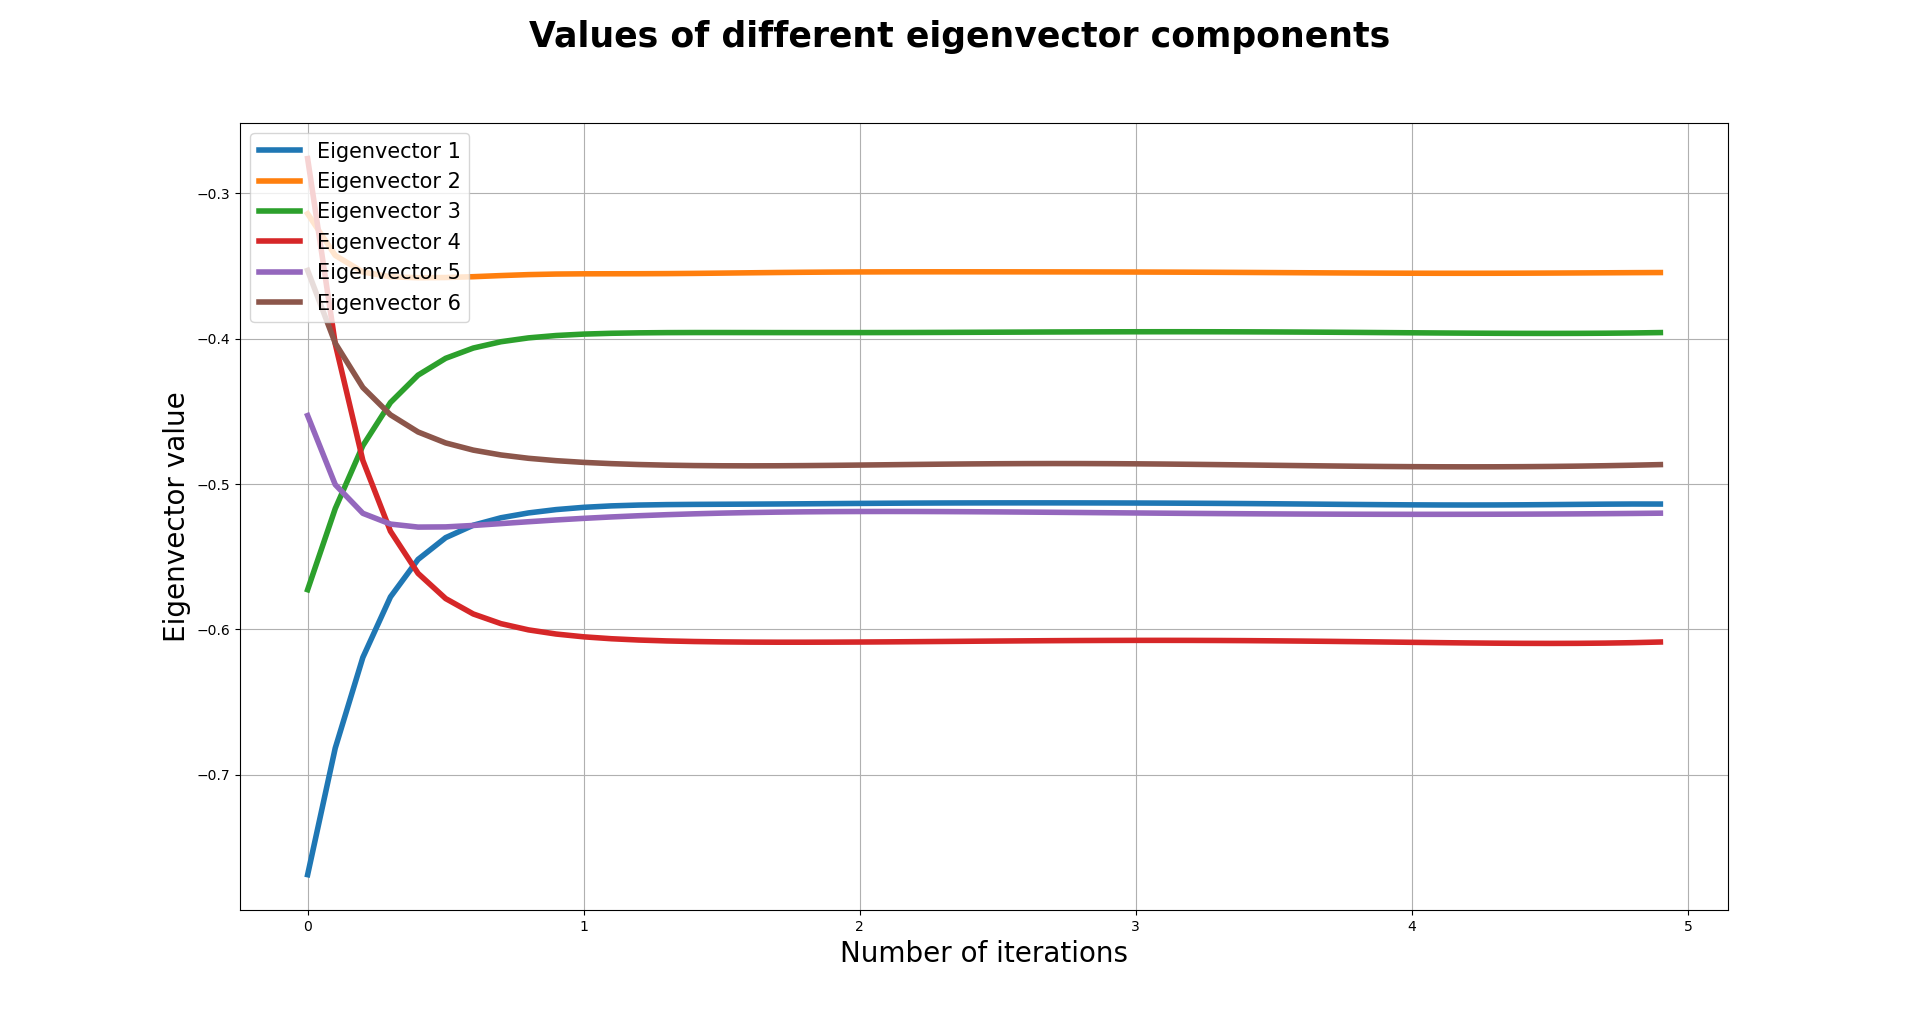
\includegraphics[width = 1\linewidth]{C:/Users/Sander/Documents/GitHub/FYS-STK4155/Project3/Report/Figures/eigen1.PNG}
\caption{\label{fig:eigen1} Convergence of the components of the eigenvector corresponding to the smallest eigenvalue. The Adam optimizer is stopped once the error of the cost function is below $0.00001$.}
\end{figure}

\noindent One can observe from figure \ref{fig:eigen1} that the components of $\nu_{min}$ quickly converges towards its correct values. However, the eigenvector components are very sensitive, so many iterations were needed to obtain the minimum eigenvalue ($720244$ to be exact). The error of the cost function after these iterations were found to be $9.9941 *10^{-6}$.
\\
We can compare the smallest eigenvector and eigenvalue to the one found by numpy with the function numpy.linalg.eig as seen in below.

\begin{equation}\label{eq:numpyEigenVec}
\nu_{min,norm,numpy} = [-0.43040961, -0.78866792, 0.177719, -0.23351243, 0.31853479, -0.07193036]
\end{equation}

\begin{equation}\label{eq:numpyEigenVal}
\lambda_{min,numpy} = 3.1220782539801926
\end{equation}

\noindent It is first observed that the minimum eigenvalue produced from the neural network is very close to the minimal eigenvalue produced by the numpy algorithm. However, the eigenvectors are different from one another. This is caused by the minimal eigenvalue having a multiplicity of at least 2 such that the two eigenvectors in equations \ref{eq:minEigenVecNorm} and \ref{eq:numpyEigenVec} are linearly independent (Axler, 2015). 

\newpage

\begin{center}
\Large{\textbf{Exercise e): Discussion}}
\end{center}

\begin{center}
\large{\textbf{Comparing the analytical, forward Euler and neural network solutions to the heat equation}}
\end{center}

\noindent We first compare the results from the analytical, forward Euler and neural network solutions to the heat equation. The following comparison then assumes the analytical solution is the correct solution to the heat equation. This statement is not entirely correct there exists some assumptions in the derivation of the solution of the heat equation (between equation \ref{eq:sumN} and \ref{eq:finalSol}). Even still, the analytical solution is deemed the correct solution. 
\\
One observed from comparing figures \ref{fig:rodHeatEulerT0DX01}, \ref{fig:rodHeatEulerT05DX01} and \ref{fig:rodHeatEulerT1DX01} to figures \ref{fig:rodHeatEulerT0DX001}, \ref{fig:rodHeatEulerT05DX001} and \ref{fig:rodHeatEulerT1DX001} that the forward Euler approaches the analytical solution more and more as the step size in space (and therefore also step size in time due to $\frac{\Delta t}{\Delta x^2} < 0.5$) approaches zero. This is due to the forward Euler approach being rooted in the definition of the derivative, meaning that smaller step sizes leads to a better approximation of the true derivative. Furthermore, the forward Euler using a step size in space of $0.001$ is equivalent to the analytical solution at all times.
\\
The neural network solution is also equivalent to the analytical solution for $t = 0$ (initial heat distribution) and $t = 0.5$. However, the neural network implementation deviates from the analytical solution at $t = 1$. This was a recurring problem with the neural network implementation for later times, as the trained model was unable to reduce the cost function below a certain threshold. Because of this and the fact that the temperature is very low at later times, means that deviations from the analytical solution occurs at later times.
\\
It was shown here that both the forward Euler and neural network implementations can solve the one dimensional heat equation. It is difficult to extrapolate this to further dimensions. However, Koryagin et.al. showed that it is possible to solve the two dimensional heat equation using a similar dense layer neural network as done here (Koryagin et.al., 2019). We also know that the two dimensional heat equation has an analytical solution and can be solved using forward Euler. However, when the system gets more complicated than this, the neural network should still be able to yield an approximate solution where the forward Euler cannot. Such a neural network may be the deep Euler method (Xing and Cheng, 2020). However, this method have mostly been tested on ordinary differential equations (the heat equation is a partial differential equation), but there may be possibility of utilizing this method on PDEs as well. 

\begin{center}
\large{\textbf{The lowest eigenvector/value of a real, symmetric and randomly generated square matrix}}
\end{center}

\noindent The neural network code, with a few adjustments, were also able to find the smallest (also highest could be achieved) eigenvalue of a real, symmetric and randomly generated square matrix. One can observe that the eigenvalues from my own neural network in equation \ref{eq:minEigenVal} is almost identical to the one that numpy achieves in equation \ref{eq:numpyEigenVal}. However, the eigenvectors are different as can be observed from equation \ref{eq:minEigenVecNorm} and \ref{eq:numpyEigenVec}. This is due to the multiplicity of the eigenvalue where multiple different eigenvectors can produce an eigenvalue (Axler, 2015). This means that the results from the paper by Yi and Fu (Yi and Fu, 2004) are reproducible. 
\\
The paper do not cover how to obtain the eigenvalues that are not the minimum/maximum eigenvalues, but there are other methods to obtain these. However, it has been proven, both in the paper by Yi and Fu and in this project, that a neural network implementation can find the minimum and maximum values of a real, symmetric and square matrix.

\newpage

\begin{center}
\Large{\textbf{Conclusion}}
\end{center}

\noindent a

\newpage

\begin{center}
\Large{\textbf{Future work}}
\end{center}

\noindent a

\newpage

\begin{center}
\Large{\textbf{References}}
\end{center}

\begin{itemize}
	\item Axler, S., 2015, \emph{Linear Algebra Done Right}, Third Edition, Springer International Publishing, page 136, Available from: \href{{https://zhangyk8.github.io/teaching/file_spring2018/linear_algebra_done_right.pdf}}{\nolinkurl{https://zhangyk8.github.io/teaching/file_spring2018/linear_algebra_done_right.pdf}}, DOI 10.1007/978-3-319-11080-6
  \item Hancock, M. J., 2006, \emph{The 1-D Heat Equation, Linear Partial Differential Equations}, page 5, Available from \href{{https://ocw.mit.edu/courses/mathematics/18-303-linear-partial-differential-equations-fall-2006/lecture-notes/heateqni.pdf}}{\nolinkurl{https://ocw.mit.edu/courses/mathematics/18-303-linear-partial-differential-equations-fall-2006/lecture-notes/heateqni.pdf}}
  \item Kingma, D. P., Ba, J. L., 2014 \emph{Adam: A Method for Stochastic Optimization}, pp 1, arXiv:1412.6980v9
  \item Koryagin, A., Khudorozkov, R., Tsimfer., S., 2019, \emph{PYDENS: A PYTHON-FRAMEWORK FOR SOLVING DIFFERENTIAL EQUATIONS WITH NEURAL NETWORKS}, Available from: \href{{https://arxiv.org/pdf/1909.11544.pdf}}{\nolinkurl{https://arxiv.org/pdf/1909.11544.pdf}}
  \item Xing, S., Cheng, X., 2020, \emph{Deep Euler method: solving ODEs by approximating the local truncation error of the Euler method}, Available from: \href{{https://www.researchgate.net/publication/340180255_Deep_Euler_method_solving_ODEs_by_approximating_the_local_truncation_error_of_the_Euler_method}}{\nolinkurl{https://www.researchgate.net/publication/340180255_Deep_Euler_method_solving_ODEs_by_approximating_the_local_truncation_error_of_the_Euler_method}}
  \item Yi, Z., Fu, Y., 2004, \emph{Neural Networks Based Approach Computing Eigenvectors and Eigenvalues of Symmetric Matrix}, Available from: \href{{https://www.sciencedirect.com/science/article/pii/S0898122104901101}}{\nolinkurl{https://www.sciencedirect.com/science/article/pii/S0898122104901101}}
\end{itemize}

\end{document}
